% Excellent overview of low-mass stars for the introduction chapters:
% https://arxiv.org/pdf/1804.04133.pdf


\chapter{Introduction}\label{chapter:introduction}


% greate review by https://arxiv.org/pdf/1610.05765.pdf
\iffalse
\begin{quote}
``{\it Only two things are infinite, the universe and human stupidity, and I'm not sure about the former.}''

-- Albert Einstein
\end{quote}
\fi

% Introduction to the M-spectral type
When you observe the night sky with only your eyes none of the stars you see will be M-dwarfs, yet they are the most common stars in the galaxy making up over 75\% of all stars\footnote{Updated counts provided at www.reons.org} \cite{2006AJ....132.2360H}. Some stars you will see are of the spectral type M, but these are giant stars which have evolved and swelled to the point in which their outer-layers have cooled. These are called M-giants and can be easily seen with a reddish twinkle in the night-sky; an example is Betelgeuse which is North-East of Orion's belt in the northern hemisphere. One thing the M-dwarfs/giants share is outer layers cool enough to permit opacities from diatomic molecules ($T_{\rm eff} \approx 3000$\,K). If you were to split the visible light from an M-dwarf with a prism you would see large absorption bands corresponding to titanium-oxide (TiO), calcium-monoxide (CO) and water (H$_2$O). These signatures denote an M-type star by the classical Harvard spectral classification scheme. 

Despite the observational similarities, M-dwarfs and M-giants differ when you peer below the outer layers. Betelgeuse probably started its life as a $20$-$M_{\odot}$ O-type main-sequence star, the exact mass depending on an assumed initial rotation, parallax measurement and which stellar models you employ \cite{2013EAS....60..307V}. Internally, Betelgeuse's hydrogen core has collapsed and brought in more hydrogen resulting in shell burning around the core. This results in a swelling of the outer layers lowering the surface temperature (giving Betelgeuse it's reddish glint and spectral type) but increasing it's overall luminosity. During this phase Betelgeuse underwent short periods of heavy mass-loss and developed an extended atmosphere \cite{2014Natur.512..282M}. M-dwarfs lead much less flamboyant lives, but are anything but boring.




\section{Properties of M-dwarfs}

% evolution PMS through MS
 M-dwarfs form like any other star; a cloud of gas and dust clumps together by means of gravity and begins rotating. A potential source of energy comes from the gravitational potential released when such contraction occurs in the pre-main sequence (PMS). The virial theorem informs us that only half of the change in gravitational energy is available to be radiated away upon contraction; the rest heats the internal gas. It is possible to calculate\footnote{https://www.ast.cam.ac.uk/~pettini/STARS/Lecture07.pdf} the energy released assuming a radial density distribution,
%
\begin{equation}\label{virial_energy}
    \Delta E_g = \frac{3}{10} \frac{G M_\star^2}{R_\star},
\end{equation}
%
where $M_\star$ is the mass of the star, $R_\star$ is the radius and $G$ is the gravitational constant. For the Sun, $\Delta E_g \approx 1.2 \times 10^{48}$\, erg (1\,erg = $10^{-7}$\,J). If a star radiates at a luminosity $L_\star$, the \textit{Kelvin-Helmholtz} timescale can be calculated,
%
\begin{equation}\label{kelvin_helmholtz_timescale}
    \tau_{\rm KH} = \frac{\Delta E_g}{L_\star}.
\end{equation}
%
This is essentially the time taken for a protostar to reach the zero-age main-sequence (ZAMS). Contraction is slowest when both $R_\star$ and $L_\star$ are small ($\tau_{\rm KH} = \Delta E_g / L_\star$ and $\Delta E_g \propto 1/R_\star$) and thus the PMS lifetime of an M-dwarf is largely spent in the final stages of contraction. For example, a 0.35\,$M_\odot$ M-dwarf remains in the PMS phase for approximately 0.18\,Gyr.\footnote{Estimated using MESA evolutionary tracks (\citealt{2016ApJS..222....8D},\citealt{2016ApJ...823..102C}) for a M-dwarf with $M = 0.3$\,$M_\odot$ at solar metalicity.} In the Solar case $\tau_{\rm KH} \sim  10^{7}$\,yr, which is two orders of magnitude smaller than the age of the solar system measured measured from radioactive dating (e.g. \citealt{2005Natur.436.1127B}).

Kelvin-Helmholtz contraction and late-stage accretion increase the young M-dwarf's angular momentum. However, interactions with the protostellar disk counteract this and reduce the M-dwarfs angular momentum \citep{2005ApJ...632L.135M}.  Eventually, the protostellar disk is cleared and the M-dwarf enters the main sequence (MS) where few drastic changes will occur. During this phase subsequent spin-down is caused by magnetised winds carrying away angular momentum \citep{2003ApJ...586..464B}. For FGK dwarfs older than 500\,Myr, the loss of angular momentum is predictable ($\propto t^{-0.5}$) leading to the field of \textit{gyrochronolgy}: predicting a stars age from its rotation rate \citep{2008ApJ...687.1264M}. Using gyrochronology for M-dwarfs is not so straightforward. Below the convective limit there appears to be two distinct populations of faster and slower rotators ($P_{\rm rot} < 10$\,d and $P_{\rm rot} > 70$\,d; \citealt{2011ApJ...727...56I}; \citealt{2016ApJ...821...93N}) making it difficult to determine the age of M-dwarfs from rotation alone. This gap likely originates from a short and rapid loss of angular momentum \citep{2011ApJ...727...56I}. M-dwarfs ultimately reach a rotational period of $> 100$\,d at a typical age of 5\,Gyr \citep{2016ApJ...821...93N}. A further indicator of age comes from H$\alpha$ emission with coincidental X-ray emission in M-dwarfs \citep{2007AJ....134.2398C}. These indicators mark the presence and strength of magnetic fields which are intertwined with age and rotation (\citealt{2006AJ....132.2507W}, \citealt{2008AJ....135..785W}).

A scaling argument used by \citet{2016PhR...663....1S} states that a star's main-sequence lifetime scales as $M_\star / L_\star$, where $L_\star \sim M_\star^3$ for low-mass stars \citep{2009itss.book.....P}. A 0.1-$M_\odot$ star is therefore expected to stay on the main sequence 100 times longer compared to the Sun. In reality however, this factor is more like 1000 due to additional sources of longevity unique to M-dwarfs. The first is slower rate of fusion as a consequence of a cooler core temperature. The second stems from the (almost) fully-convective nature of M-dwarfs. This replenishes hydrogen in the core which is being fused via the P-P chain whilst simultaneously preventing He ash building up. M-dwarfs therefore have access to almost all of their hydrogen to burn \citep{2004RMxAC..22...46A} compared to Solar type stars which are restricted to hydrogen in the core (about 10\%; \citealt{2016PhR...663....1S}). The combined effect extends the MS lifetime of M-dwarfs well in excess of Hubble time ($\sim 200$\,Gyr; \citealt{1998A&A...337..403B}).


% spectral type
\begin{figure}
    \centering
    \includegraphics[scale=0.5]{3-images/M_dwarf_spectra.png}
    \caption{Illustrative example of spectra for an inactive M1 star and an active M6 star with strong molecular and atomic feautures labelled. Taken from \protect\citet{2007AJ....133..531B}.}
    \label{fig:M6_spectra}
\end{figure}

The spectral type of an M-dwarf is generally estimated by comparing its spectrum to a set of benchmark spectra (e.g. \citealt{2007AJ....134.2398C}). The spectral type M is defined by strong moleculer absorption from titanium oxide (TiO) blueward of the optical ($\sim$450-570\,nm; \citealt{morgan}). Molecular opacity from diatomic hydrogen (H$_2$), water (H$_2$O) and vanadium oxide (VO) obscure the continuum making the task of determining atmospheric parameters a subtle endeavour (see Fig. \ref{fig:M6_spectra}). The classification of M-dwarf boundaries is subject to the quirks of astronomical history. For example, strong TiO lines can be measured at redder wavelengths for stars hotter than M0 but required the development of red-sensitive detectors at the end of 20$^{th}$ century (\citealt{1991ApJS...77..417K}, \citealt{1991AJ....101..662B}). 

The lower limit of the M spectral type is M7/M8 (the hydrogen burning limit; \citealt{1998A&A...337..403B}). Determining spectral types for stars in this regime is challenging as small mass and metallicity variations result in physical changes which move objects from one category to another \citep{2014AJ....147...94D}. Young brown dwarfs look almost identical to late M-dwarfs and requires diligent analysis of the atmosphere to discern the two. For example, molecules like ammonia or methane can only survive at colder temperatures ($\sim 1000$\,K; \citealt{1999A&A...349L..41C}) pointing towards a brown-dwarf. Brown dwarfs are also distinguished by their inability to fuse hydrogen, but they can fuse less abundant isotopes like deuterium and lithium. A further complication arises from spectral types as late as L2 occasionally possessing the minimum mass required for hydrogen fusion to occur \citep{2014AJ....147...94D}. 



    
\section{Absolute parameters of low-mass stars}
    
% Paragraph 1
%---------------------
% determining absolute parameters of M-dwarfs not easy
% Such measurements provide crucial tests to evolutionary models at the bottom of the main sequence which feed into our understanding of planets found around them.
% The frequently use quote ”know thy planet, know thy star” is pertinent for low-mass stars as exitement surrounding them grows.

% Paragraph 2 (INTEFER)
%---------------------


% exists some tension between absolute parameters predicted by stellar models
% M-dwarfs appear systematically higher radius than predicted by evolutionary models from interferometry



\subsection{Interferometry}

M-dwarfs may be monitored simultaneously through two or more telescopes. The light from these instruments can be combined to produce an interference pattern of alternating light and dark bands. The most common measurement in optical and infrared interferometry is a measurement of the amplitude of the fringes. This fringe contrast is often called the ``\textit{visibility}'' of the fringes.  The normalised visibility amplitude ($V$) is computed from the maximum and minimum intensity ($P$) of the fringes, given by
%
\begin{equation}
V = \frac{P_{max} - P_{min}}{P_{max} + P_{min}}.
\end{equation}
%
An unresolved point source will have a normalised visibility amplitude of 1.  For a spatially resolved star, light from across the stellar surface combines incoherently causing the visibility amplitude to be less than 1.  The bigger the star, the smaller the fringes and lower the fringe amplitude.  By measuring this drop in the fringe amplitude it is possible to measure the size (angular diameter), shape, and surface features of an M-dwarf. Accurate parallax measurements also permit a measurements of the effective temperature. A binary star will produce two fringe packets, one for each star in the system.  If the separation between the stars is small enough, the fringe packets from each star will overlap, producing a periodic signal in the visibility amplitudes.  The separation between the peaks in the visibility curve provides a measurement of the binary separation while the minimum visibility reflects the flux ratio between the components. 

There have been many successful attempts to measure the radius and temperature of single M-dwarfs (e.g. \citealt{1997A&A...325..159L}, \citealt{2006ApJ...644..475B}; \citealt{2001AAS...198.5120N}; \citealt{2003A&A...397L...5S}; \citealt{2009A&A...505..205D};  \citealt{2012ApJ...757..112B}; \citealt{2015csss...18..839V}). The fraction of M-dwarfs which have companions within 1000\,AU is estimated to be $\sim$40\% (\citealt{1992ApJ...396..178F}; \citealt{2006ApJ...640L..63L}; \citealt{2010ApJS..190....1R}). If the systems is close and bright enough, interferometry can monitor the relative positions of each component $\Delta \alpha$, $\Delta \delta$) relative to the centre of mass. An example is given by \citet{2016AJ....152..141B} who used white-light interferometric observations from the Hubble Space Telescope with radial velocity data from the McDonald Observatory to obtain astrometric solutions of M-dwarfs in binary systems. They achieved mass uncertainties as low as 0.4\% in some cases (median error of 1.8\%), but the radius of each component remained poorly constrained.

%Those which have radius and temperature measurements demonstrate a significant tension between observations and stellar models. \citet{2012ApJ...757..112B} acquired interferometric observations at the CHARA Array in the near-infrared $K'$ and $H$ bands \citep{2005ApJ...628..453T} for 21 nearby, single and bright red dwarfs. They measured radii with an uncertainty below 3\% and uncertainty in $T_{\rm eff}$ below 1\% and robustly demonstrate that models over-predict $T_{\rm eff}$ by $\sim3\%$, and under-predict radii by $\sim5\%$. Obtaining the mass for single stars often requires photometric calibrations for red-dwarfs (e.g. \citealt{1993AJ....106..773H}; \citealt{2000A&A...364..217D}; see Sect. \ref{introduction:luminosity_relations}). The uncertainty associated with these relations can be up to $10\,\%$ which makes it difficult to test evolutionary models. 



% DEBs
% M+M binaries
\subsection{Eclipsing binaries}

Eclipsing binarys can be used to measure absolute parameters of M-dwarfs. The drop in light as one companion occults another  sets the scale of radii for each component. Binary companions of equal luminosity have spectral features that can be attributed to individual components. This may permit a measurement of temperature and radial velocity for each star from a single spectrum. Radial velocity measurements at numerous points in an orbit characterises the \textit{spectroscopic orbit} which sets the mass scale of the system. Eclipsing binaries where both spectra are discernible are called double-lined eclipsing binaries (SB2s). These systems allow a measurement of the absolute parameters of each star. In John Southworth's catalogue of well-studied detached eclipsing binaries \citep{2015ASPC..496..164S} there are 11 systems%
\footnote{Accessed 25$^{th}$ Oct 2018.}
%
in which both systems have the M-spectral type (\citealt{2010ApJ...712.1003W}, \citealt{2002ApJ...567.1140T}, \citealt{2011ApJ...728...48K}, \citealt{2018AJ....155..114H}, \citealt{2003A&A...398..239R}, \citealt{2017ApJ...845...72K}, \citealt{2011ApJ...742..123I}, \citealt{2016ApJ...816...21D}, \citealt{2016ApJ...816...21D}). Systems where only one spectral component can be measured are called single-lined eclipsing binaries (SB1s) and require supplementary information to determine some absolute parameters (e.g. masses and radii). A more in-depth theory of eclipsing binaries is given in Sect. \ref{chapter:theory}.

A different approach is to measure the absolute parameters of eclipsing binary systems where only one of the stars is an M-dwarf. One such example is M-dwarf + white-dwarf systems. The small size of the white-dwarf ($R \sim 1\,R_\oplus$) results in very sharp, total eclipses which can be used to measure radii to a precision of a few percent  \citep{2010MNRAS.402.2591P}. Consequently, it is possible to obtain a clean M-dwarf spectrum free from contamination of the white dwarf. The cooling of white dwarfs is well understood (e.g. \citealt{1997ApJ...486..413S}, \citealt{2013A&A...555A..96S}, \citealt{2014Natur.515...88V}) making them ideal systems to determine the age of an M-dwarf. These systems have experienced a brief common envelope phase when the progenitor star to the white dwarf evolved off the main sequence. This has a negligible effect on the M-dwarf as the common envelope phase is short (0.001-0.01\,Myr) compared to the thermal timescale of the M-dwarf (0.1-1\,Gyr). Additionally, the common envelope has a much higher specific entropy than the surface of an M-dwarf so very little accretion will take place \citep{1991ApJ...370..709H}.



\section{Tension with stellar models}\label{introduction:tension}


\begin{figure}
    \centering
    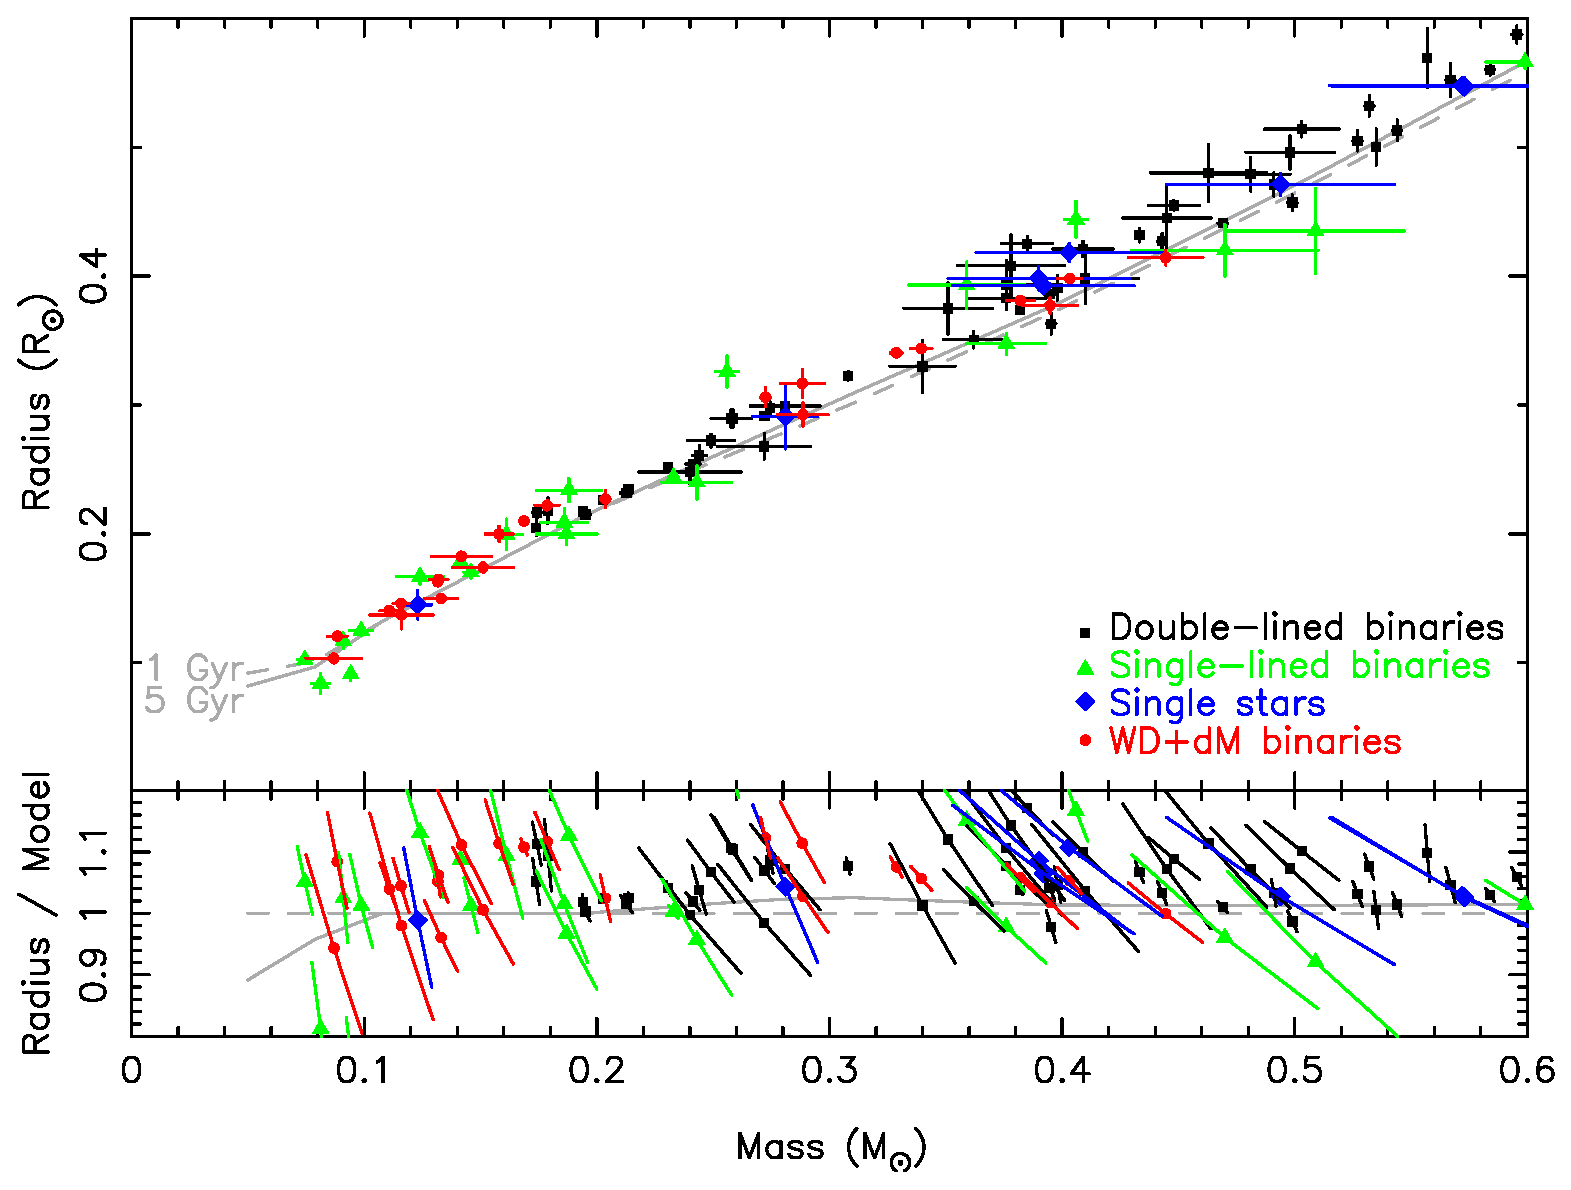
\includegraphics[width=\textwidth]{3-images/MDMR.eps}
    \caption{Mass-radius plot for low-mass stars (with mass and radius uncertainties of less than 10 per cent). The type of system that the measurement came from is indicated by the different colours and symbols and all are detailed in either Table 2 (red points) or the Appendix (all other points) of \protect\citet{2018MNRAS.481.1083P}. Also shown are the theoretical mass-radius tracks from \protect\citet{2003IAUS..211...41B}; \protect\citet{2015A&A...577A..42B}. Image taken from \protect\citet{2018MNRAS.481.1083P}}.
    \label{introduction:fig:parsons}
\end{figure}


There is an emerging tension between measurements of mass, radius and temperature compared to what is predicted from evolutionary models. M-dwarfs across the spectral type are reported to have a radius 5\% higher than expected (\citealt{2000ApJ...542..464C}; \citealt{2002ApJ...567.1140T}; \citealt{2003A&A...398..239R}; \citealt{2005ApJ...631.1120L}; \citealt{2008MmSAI..79..562R}; \citealt{2014ApJ...797...31T}; \citealt{2015A&A...577A..42B}; \citealt{2017ApJ...844..134L}). Some also have temperature hotter than predicted (\citealt{2012MNRAS.423L...1O}, \citealt{2014A&A...572A..50G}). The most glaring discrepancies are measured for low-mass stars near the convective transition ($\sim 0.35$M$_\odot$; \citealt{2007ApJ...660..732L}). The disparity also seems to be equally evident in single M-dwarfs and those in eclipsing binaries (Fig. \ref{introduction:fig:parsons}; \citealt{2013ApJ...776...87S}). A recent discovery of an over-luminous late-type M-dwarf around a solar-like star, CWW 89Ab ($\sim 0.035 M_\odot$; \citealt{2018AJ....156..168B}) suggests that this problem could extend into the brown-dwarf region. There are a few competitive theories circulated in the literature to explain the origins of this phenomena.

\subsection{Magnetic activity}

\begin{figure}
    \centering
    \includegraphics[width=\textwidth]{3-images/spada.png}
    \caption{Radius discrepancy as a function of activity indicator in a sample of low-mass stars (below solar) measured by interferometry. Image taken from \protect\citet{2013ApJ...776...87S}.}
    \label{fig:inflation_VS_Lx}
\end{figure}

The presence of magnetic fields is often invoked to explain the systematic inflation of M-dwarfs. Enhanced magnetic fields generated by the dynamo affect the convectional stability criteria leading to larger radii for the same temperature (or vice versa; \citealt{2013ApJ...776...87S}). For low-mass stars, strong surface magnetic fields (0.01-1\,kG; see \citealt{2012LRSP....9....1R}) are generated in the convective zone via dynamo mechanisms (\citealt{2013SAAS...39..187C}; \citealt{2001ApJ...559..353M}). In eclipsing binary systems, low-mass stars can be coerced into a regime of fast rotation which enhances dynamo mechanisms leading to increased magnetic activity. Stabilisation of convection in stellar models can reproduce the observed radius inflation of fully-convective M-dwarfs with reasonable surface magnetic fields, but require super-MG magnetic fields in the interior \citep{2014ApJ...789...53F}. As noted by \citet{2014ApJ...789...53F}, the presence of such a strong internal magnetic fields is unlikely for a number of reasons: turbulent dynamos in convective regimes cannot generate magnetic fields in excess of 50\,kG (\citealt{2006ApJ...638..336D}, \citealt{2008ApJ...676.1262B}) and there is no mechanism describing how MG magnetic fields would accumulate in the interior of convective stars. 
        
\citet{2005ApJ...631.1120L} conjectured that spots may explain the enhanced radius measured for GU Bootis. Star spots are manifestations of suppressed surface convection brought upon by magnetic fields. They have the effect of creating regions of different temperatures on the stellar surface; they can shift stars bluer or redder depending on there density, location, temperature differences and the photometric colours used \citep{2013ApJ...779..183F}. Significant spot coverage has the effect of lowering the overall photospheric temperature. To maintain radiative equilibrium, a star must increase its radius to conserve total flux output.  If this were to be the case, we would see a clear trend of inflation with magnetic indicators (e.g. H$\alpha$ emission, X-ray emission), rotation and age. Work by \citet{2013ApJ...776...87S} found activity indicators were independent of inflation for single and binary M-dwarfs (see Fig. \ref{fig:inflation_VS_Lx}). Significant inflation has been observed for both short period (e.g., KOI-126, $P_{\rm orb} = 1.77$\,d; \citealt{2011Sci...331..562C}) and long period systems (e.g., Kepler-16, $P_{\rm orb} = 41.1$\,d; \citealt{2011Sci...333.1602D}; \citealt{2011ApJ...737L..18W}) making it unclear whether tidally-induced magnetic fields can be blamed. 
        

\subsection{Metalicity}

\begin{figure}
    \centering
    \includegraphics[scale=0.5]{3-images/berger.png}
    \caption{Fractional deviation between the radii measured through long baseline optical interferometry and from the model predictions for stellar radius from \protect\citet{1997A&A...327.1039C} plotted as a function of metalicity. Measurements include long-baseline interferometry (filled symbols) and spectrophotometry of eclipsing binaries (open circles). The interferometry data included are from this paper (circles), PTI (\protect\citealt{2001ApJ...551L..81L}, triangles), and VLTI (\protect\citealt{2003A&A...397L...5S}, squares). The representative errors are $\pm0.2$ dex in [Fe/H] and $\pm0.1$ in fractional deviation of the radius (due to 10\% errors in the mass estimates). Image take from \protect\citet{2006ApJ...644..475B}.}
    \label{fig:berger_inflation}
\end{figure}


\begin{figure}
    \centering
    \includegraphics[scale=0.5]{3-images/Demory.png}
    \caption{Fractional deviation of single stars radii derived by interferometry  \protect\citep{1998A&A...337..403B} vs. stellar metallicity. Image take from \protect\citet{2009A&A...505..205D}.}
    \label{fig:demory_inflation}
\end{figure}

\citet{2006ApJ...644..475B} used the CHARA array to measure the radius M-dwarfs using interferometry. In their figure 5 (Fig. \ref{fig:berger_inflation}) there exists a clear trend between a stars metalicity and fractional radius residual, with less inflation observed for metal-poor stars. The same conclusion is found by \citet{2000ApJ...535..965L} and \citet{2007ApJ...660..732L} who used spectral fits to determine a systematic inflation in stars with higher metalicity. 
%Metalicity is closely related to stellar opacity and structure, and missing opacity, such as TiO, would explain an underestimation of radii for some M-dwarfs. 
However, more recent results from \citet{2009A&A...505..205D} which excluded measurements from  \citet{2006ApJ...644..475B} no longer show this trend (Fig. \ref{fig:demory_inflation}). It is likely that metallicity plays some role in inflation due to its direct affect on stellar structure. The accuracy and uncertainty of spectroscopic techniques is often questioned in \textit{hare-and-hounds} experiments which reveals significant discrepancies in stellar atmospheric parameters from identical spectra \citep{Jofre2016}. 

    
    
    
    
    



























% should be around 3 pages

%%%%%%%%%%%%%%%%%%%%%%%%%%%%%%%%%%%%%%%%%%%%%%%%%%%%%%
% Section 1. 

% P1
% - M-dwarfs are becoming popular exoplanet hosts
% - High probability of habitable zone transit

% P2
% - Number of M-dwarf exoplanets
% - Popular exoplanets

% P3
% - M-dwarf exoplanet atmospheric chemistry
% - Key chemicals
% - Influence from host on e
%%%%%%%%%%%%%%%%%%%%%%%%%%%%%%%%%%%%%%%%%%%%%%%%%%%%%%











%M-dwarfs are promising targets for exoplanet surveys. At a given distance, $a$, from a star of radius $R_\star$, an exoplanet (of radius $R_p$) is less likely to transit an M-dwarf than a K-/F-dwarf as the transit probability scales as ∼ $R_\star /a$. Conversely, we find that exoplanets in habitable zones are more likely to transit an M-dwarf than a larger star due to $a$ decreasing faster than $R_\star$ as we consider less massive stars. The transit depth of an eclipse scales as $(R_p/R_\star)^2$ so a similar planet will produce a deeper eclipse for a lower-mass star. An M-dwarf's low luminosity results in a habitable zone which is much closer to the sun than solar-type stars. If finding exoplanets in the M-dwarf habitable zone is the goal, then there is an increased geometric probability of observing a transit as well as number of transits observed in a given time period \citep{2008PASP..120..317N}. 

%Over the past decades there has been major progress in finding exoplanets around M-dwarfs. Over 200 planets have been found around M-dwarfs (\citealt{2013A&A...551A..48A}, \citealt{2014Sci...344..277Q}, \citealt{2014ApJ...784...45R}, \citealt{2015ApJ...800...99T}, \citealt{2015ApJ...804...10C}, \citealt{2015ApJ...809....7B}, \citealt{2016ApJ...818...87S}, \citealt{2016Natur.536..437A}, \citealt{2017Natur.542..456G}). These discoveries come from radial velocity surveys, transit surveys (both ground- and space-based) along with microlensing. Of note are the discoveries of exoplanets around Trappist-1 \citep{2017Natur.542..456G} and Proxima Centauri \citep{2016Natur.536..437A} which has increased the popularity of M-dwarfs for the public and scientists alike. 

%There have been recent advances in theoretical research along with observational evidence to support the conclusion that a myriad of other factors may disrupt the traditional idea of M-dwarf habitability (instead of just a function of $a$). The intense stellar activity of an early-life M-dwarf can lead to significant alterations in atmospheric chemistry \citep{2016PhR...663....1S}. In particular, the abundances of ozone \citep{2010AsBio..10..751S}, surface water,  molecular oxygen \citep{2015AsBio..15..119L} and CO$_2$ \citep{2015ApJ...806..249G} can be modified by stellar activity. In cases where close-in planets form with thick H$_2$ envelopes, however, stellar activity could photoevaporate these envelopes unveiling habitable cores \citep{2015AsBio..15..119L}.  M-dwarf emission is stronger in the IR and near-IR and so gases that absorb there are expected to have an important contribution to the discussion of habitability. Molecules like CO$_2$, H$_2$O, CHG$_4$ and O$_3$ are able to absorb a larger fraction of flux from an M-dwarf compared to the same planet around a hotter star. Planets with dense CO$_2$ atmospheres could see an increase in surface habitability through increased surface temperature \citep{2011mamo.conf..447W}. However, at the distant end of the habitable zone the effects of Rayleigh scattering will supersede atmospheric warming by CO$_2$ leading to frozen surface conditions \citep{2016PhR...663....1S}.


%%%%%%%%%%%%%%%%%%%%%%%%%%%%%%%%%%%%%%%%%%%%%%%%%%%%%%
% Section 2. 

% P1
% - Discussion of exoplanets is limited to how well we know the host
% - know thy planet
% - We cannot accurately infer parameters about the planet since we do not 
%   fully understand.
% - Turn to empirical relations

% P2
% - Attempts to measure the mass-radius plane
% - DEBs, SEB, interfereometry, WD+M, EBLMs (discussed in Sect. X)

% P3 
% - Results from Mass radius diagram
% - inflated radii
% - Hotter than expected
% - what it means for exoplanets? 
%%%%%%%%%%%%%%%%%%%%%%%%%%%%%%%%%%%%%%%%%%%%%%%%%%%%%%


%%%%%%%%%%%%%%%%%%%%%%%%%%%%%%%%%%%%%%%%%%%%%%%%%%%%%%
% Section 2. 

% P1 
% - Motivation for the first part
% - Determine robust atmospheric parameters for FGK stars 
% - SNR usually low (<20) for CORALIE optimised for RV
% - Long term systematic trends and noise make it difficult to fit lines of measure EW

% P2 
% - Use wavelet decomposition
% - capable of discering spectral features from noise/trends
% - a fast way to estimate atmospheric parameters from spectra 

% P3
% - The second part stems for the first
% - We could measure atmospheric parameters of EBLM systems identified with WASP with spectra measured from the EBLM project
% - RVs of sufficient quality
% - oppertunity to obtain follow-up photmetry
% - Measure absolute parameters of EBLMs from the ground

% P4
% - Four EBLMs were observed with K2
% - High quality lightcurves with spotted features
% - provides an oppertunity to study EBLMs in a new way with analytical lightcurves and red-noise models
% - 
% P5
% - Lots of EBLMs which have been homogenusly studied
% - Chance to study trends emerging which point to tidal inflation
% - explore possible uncertainties from assumptions of evolutionary models and orbital fit. % - What needs to be done
% - Develop EBLM studies
%%%%%%%%%%%%%%%%%%%%%%%%%%%%%%%%%%%%%%%%%%%%%%%%%%%%%%












\iffalse
Am of this thesis:
        establishe techniqe and practabitlity of mass, radii from EBBLMs
        Towards space-based photometry
        measure the Fe to get stars which arent solar
         Target the best ones for follow-up WASP
        Bottleneck with followup
                K2 and TESS will investigate

        What needs to be done

        What techniques, can we develop them? o[timising TESS/K2 CHEOPS

        How many will we need? How precisely? 1000 at 10% or 20 at 1% 
                What is the best tactic to work out a useful relation?


towards ends, have section - aims of this thesis
        Short paragraph
        aims are to develope techniqyes to study EBLMs - apply them
        Work out a strategy for EBLM studies
                Few or many? how many? 

\fi


\iffalse
\section{Properties of M-dwarfs}

 M-dwarfs form like any other star; a cloud of gas and dust clumps together by means of gravity and begins rotating. A potential source of energy comes from the gravitational potential released when such contraction occurs in the pre-main sequence (PMS). The virial theorem informs us that only half of the change in gravitational energy is available to be radiated away upon contraction; the rest heats the internal gas. It is possible to calculate\footnote{https://www.ast.cam.ac.uk/~pettini/STARS/Lecture07.pdf} the energy released assuming a radial density distribution,
%
\begin{equation}\label{virial_energy}
    \Delta E_g = \frac{3}{10} \frac{G M_\star^2}{R_\star},
\end{equation}
%
where $M_\star$ is the mass of the star, $R_\star$ is the radius and $G$ is the gravitational constant. For the Sun, $\Delta E_g \approx 1.2 \times 10^{48}$\, erg (1\,erg = $10^{-7}$\,J). If a star radiates at a luminosity $L_\star$, the \textit{Kelvin-Helmholtz timescale} timescale can be calculated,
%
\begin{equation}\label{kelvin_helmholtz_timescale}
    \tau_{\rm KH} = \frac{\Delta E_g}{L_\star}.
\end{equation}
%
This is essentially the time taken for a protostar to reach the zero-age main-sequence (ZAMS). Contraction is slowest when both $R_\star$ and $L_\star$ are small ($\tau_{\rm KH} = \Delta E_g / L_\star$ and $\Delta E_g \propto 1/R_\star$) and thus the PMS lifetime of an M-dwarf is largely spent in the final stages of contraction. For example, a 0.35\,$M_\odot$ M-dwarf remains in the PMS phase for approximately 0.18\,Gyr.\footnote{Estimated using MESA evolutionary tracks (\citealt{2016ApJS..222....8D},\citealt{2016ApJ...823..102C}) for a M-dwarf with $M = 0.3$\,$M_\odot$ at solar metalicity.} In the Solar case $\tau_{\rm KH} \sim  10^{7}$\,yr, which is two orders of magnitude smaller than the age of the solar system measured measured from radioactive dating (e.g. \citealt{2005Natur.436.1127B}).



Kelvin-Helmholtz contraction and late-stage accretion increase the young M-dwarf's angular momentum. However, interactions with the protostellar disk counteract this and reduce the M-dwarfs angular momentum \citep{2005ApJ...632L.135M}.  Eventually, the protostellar  disk is cleared and the M-dwarf enters the main sequence (MS) where few drastic changes will occur. During this phase subsequent spin-down is caused by magnetised winds carrying away angular momentum \citep{2003ApJ...586..464B}. For FGK dwarfs older than 500\,Myr, the loss of angular momentum is predictable ($\propto t^{-0.5}$) leading to the field of \textit{gyrochronolgy}: predicting a stars age from its rotation rate \citep{2008ApJ...687.1264M}. Using gyrochronology for M-dwarfs is not so straightforward. Below the convective limit there appears to be two distinct populations of faster and slower rotators ($P_{\rm rot} < 10$\,d and $P_{\rm rot} > 70$\,d; \citealt{2011ApJ...727...56I}, \citealt{2016ApJ...821...93N}) making it difficult to determine the age of field M-dwarfs. This gap likely originates from a short and rapid loss of angular momentum \citep{2011ApJ...727...56I}. M-dwarfs ultimately reach a rotational period of $> 100$\,d at a typical age of 5\,Gyr \citep{2016ApJ...821...93N}. A further indicator of age comes from H$\alpha$ emission with coincidental X-ray emission in M-dwarfs \citep{2007AJ....134.2398C}. These indicators mark the presence and strength of magnetic fields which are intertwined with age and rotation (\citealt{2006AJ....132.2507W}, \citealt{2008AJ....135..785W}).

% Other observable signatures of activity mark the evolution of M dwarfs. The presence of Hα in emission (often coincident with X-rays in emission (Reid et al., 1995; Covey et al., 2007)) signals the presence and strength of magnetic activity and decreases with age (West et al., 2006, 2008). Across the M spectral class, the “active" duration of a star’s life varies from 1 Gyr in the case of M0 dwarfs to 8 Gyr or more for spectral type M8 (West et al., 2006).

% continue using https://arxiv.org/pdf/1610.05765.pdf

A scaling argument used by \citet{2016PhR...663....1S} states that a star's main-sequence lifetime scales as $M_\star / L_\star$, where $L_\star \sim M_\star^3$ for low-mass stars \citep{2009itss.book.....P}. A 0.1-$M_\sun$ star is therefore expected to stay on the main sequence 100 times longer compared to the Sun. In reality however, this factor is more like 1000 due to added sources of longevity unique to M-dwarfs. The first is slower rate of fusion as a consequence of a cooler core temperature. The second stems from the convective nature of M-dwarfs. This replenishes hydrogen in the core which is being fused via the P-P chain whilst simultaneously preventing He ash building up. M-dwarfs therefore have access to almost all of their hydrogen to burn \citep{2004RMxAC..22...46A} compared to Solar type stars which are restricted to hydrogen in the core (about 10\%; \citealt{2016PhR...663....1S}). The combined effect extends the MS lifetime of M-dwarfs well in excess of Hubble time ($\sim 200$\,Gyr; \citealt{1998A&A...337..403B}).
\fi


\iffalse
\section{Initial mass function}

Measuring the properties of many individual stars (e.g. from clusters) reveal their evolutionary state, age and mass. The distribution of stellar masses at birth is known as the initial mass function (IMF). The IMF has been subjected to numerous reviews (\citealt{2010ARA&A..48..339B}; \citealt{2012EAS....57...45J}; \citealt{2013pss5.book..115K}; \citealt{2014prpl.conf...53O}; \citealt{2017ApJ...841...68V}). One of the first attempts to measure the IMF determined a power-law function which decreases between 0.1-10\,$M_\odot$. However, recent studies (\citealt{2000ApJ...544.1044L};
\citealt{2000ApJ...540.1016L}; 
\citealt{2014prpl.conf...53O};
\citealt{2003PASP..115..763C};
\citealt{2006ApJ...640L..63L}) have found a break from the power law in the mass range 0.05-10\,$M_\odot$ (Fig. \ref{fig:IMF_late_stars}). 

% see 6.2 from https://arxiv.org/pdf/1402.0867.pdf
% Theories for the origin of the peak of the IMF can be divided into two groups based on what additional piece of physics they choose to add to assign a definite mass scale

There are three possible explanations which could explain this peak this peak. The first is the \textit{Jeans mass hypothesis} which states that the peak of the IMF is a reflection of the mean-density in star-forming clouds (\citealt{1992MNRAS.256..641L}, \citealt{2005MNRAS.356.1201B}) and has been applied to cosmological models (\citealt{2007ApJ...668..667T}, \citealt{2012MNRAS.423.3601N}). A serious shortcoming of this approach is the choice of scale; what should be counted as the \textit{cloud}? In simulations by \citet{2007ApJ...668..667T} and  \citet{2012MNRAS.423.3601N}, the initial speed of sound and density (which describe the Jeans mass) are entered manually, but the latter choice depends which material is traced (i.e. low-density tracer like CO or a higher one). The second potential origin invokes \textit{deviations from isothermality}. Isothermality holds only approximately for molecular clouds and such deviations may be important for setting the characteristic mass of stars (\citealt{2001BpJ....81.2020G},\citealt{2007PASJ...59..589O},\citealt{2013A&A...557A..90V}). The third mechanism involves invoking \textit{non-ideal MHD processes}. However one of the most probable process, ambipolar diffusion (the diffusion of positive and negative species due to interaction with an electric field) is not mass dependent providing the ionization fraction behaves as a power-law function of density \citep{2010ApJ...709..308M}.

Many space missions probe the IMF for the lowest-mass stars: the Spitzer space telescope \citep{2004ApJS..154....1W}, the Herschel space observatory \citep{2010A&A...518L...1P} and the wide-field infrared survey explorer (WISE; \citealt{2010AJ....140.1868W}). 
%The James Webb space telescope \citep{2006SSRv..123..485G} will further contribute to the bottom-end of the IMF.
Complimenting these are a selection of ground-based surveys which are magnitude-limited: the Two Micron All Sky Survey \citep{2006AJ....131.1163S}, the Sloan Digital Sky Survey (SDSS; \citealt{2000AJ....120.1579Y}) and the Visible and Infrared Survey Telescope for Astronomy (VISTA; \citealt{2001ASPC..232..339E}). An important conclusion from decades of probing the IMF is that low-mass stars ($\leq 0.6\,M_\sun$)form 70\% of the total stellar systems within a distance of 10\,pc \citep{2006AJ....132.2360H}.  


\begin{figure}
    \centering
    \includegraphics{3-images/IMF.png}
    \caption{The IMF $\xi(\log m) = dn/d\log m$ of stars in the Orion Nebula Cluster as inferred from \textit{Hubble Space Telescope} photometry. In each panel the black points show the data; the error bars are the 1$\sigma$ errors that result from a combination of counting statistics and incompleteness. Although the underlying data in each panel are the same, the three panels show the results of converting the observed colours and magnitudes to stellar masses using three different models. The bottom panel uses the models of \citet{1998ASPC..134..442D}, while the top two panels both use the models of \citet{1998A&A...337..403B}, using two different methods for handling stars that fall outside Baraffe et al.'s model grid. The red solid and dashed lines are the single-star and system IMFs of \citet{2003PASP..115..763C}, while the black curve is the best fit of the data to a lognormal functional form; the yellow band shows the $1\sigma$ uncertainty on the fit. Taken from  \citet{2012ApJ...748...14D}. }
    \label{fig:IMF_late_stars}
\end{figure}


\fi


%\section{The M spectral type}\label{spec_analysis_M_dwarf}

% sect. 2.1 from https://arxiv.org/pdf/1610.05765.pdf
% sect. 2.3 from https://arxiv.org/pdf/1610.05765.pdf

%The spectral type of an M-dwarf is generally estimated by comparing its spectrum to a set of benchmark spectra (e.g. \citealt{2007AJ....134.2398C}). The spectral type M is defined by strong moleculer absorption from titanium oxide (TiO) blueward of the optical ($\sim$450-570\,nm; \citealt{morgan}). Molecular opacity from diatomic hydrogen (H$_2$), water (H$_2$O) and vanadium oxide (VO) obscure the continuum making the task of determining atmospheric parameters a subtle endeavour (see Fig. \ref{fig:M6_spectra}). The classification of M-dwarf boundaries is subject to the quirks of astronomical history. For example, strong TiO lines can be measured at redder wavelengths for stars hotter than M0 but required the development of red-sensitive detectors at the end of 20$^{th}$ century (\citealt{1991ApJS...77..417K}, \citealt{1991AJ....101..662B}). 

%The lower limit of the M spectral type is M7/M8 (the hydrogen burning limit; \citealt{1998A&A...337..403B}). Determining spectral types for stars in this regime is challenging as small mass and metalicity variations result in physical variations capable of moving objects from one category to another \citep{2014AJ....147...94D}. Young brown dwarfs look almost identical to late M-dwarfs and requires diligent analysis of the atmosphere to discern the two. For example, molecules like ammonia or methane can only survive at colder temperatures ($\sim 1000$\,K; \citealt{1999A&A...349L..41C}) pointing towards a brown-dwarf. Brown dwarfs are also distinguished by their inability to fuse hydrogen, but they can fuse less abundant isotopes like deuterium and lithium. A further complication arises from spectral types as late as L2 occasionally possessing the minimum mass required for hydrogen fusion to occur \citep{2014AJ....147...94D}. 

%\begin{figure}
 %   \centering
 %   \includegraphics[scale=0.5]{3-images/M_dwarf_spectra.png}
%    \caption{Illustrative example of spectra for an inactive M1 %star and an active M6 star with strong molecular and atomic %feautures labelled. Taken from %\protect\citet{2007AJ....133..531B}.}
%    \label{fig:M6_spectra}
%\end{figure}


%\begin{figure}
 %   \centering
%    \includegraphics{3-images/CaH2_fig_2_PASP_118_840_218.jpg}
%    \caption{Temperature vs. CaH2 index for program stars from \protect\citealt{2006PASP..118..218W}. The line is a least‐squares fit: Teff = (2696 + 1618 × CaH2) K. Image taken from Fig.2 of \protect\citealt{2006PASP..118..218W}.}
%    \label{fig:CaH2_index}
%\end{figure}

%Currently there are no robust ways of measuring metalicity from low-resolution spectra of M dwarfs \citep{2008AJ....135..785W}. It is possible to use calibrated molecular indices to measure an M-dwarf metalicity using measurements of equivalent widths from atomic lines in high-resolution spectra ($\lambda / \Delta \lambda \approx 33,000$; \citealt{2008AJ....135..785W},\citealt{2007AJ....134..778M}). Despite their abundance in the Galaxy, their faintness thwarts obtaining high resolution spectra of more distant M-dwarfs and thus an alternate method is required. Low resolution spectra ($R \approx 3000$) can go approximately 3 mag. fainter ($V \geq 16$ for a 4-m class telescope) and permits the measurements of molecular indices. Two such are the CaH2 and TiO5 indices which measure CaH and TiO band strengths respectively. CaH2 is strongly correlated with photospheric temperature (see Fig. \ref{fig:CaH2_index}). TiO5 depends on temperature and metalicity: for a given temperature or CaH2 value, a smaller TiO5 value indicates a smaller metallicity. Measuring $\log g$ can be done using the unblended FeH lines in the infrared with careful treatment micro-/macro-turbulence \citep{2009AIPC.1094..816W}. The alkali lines also show large wing variations due to pressure broadening. The K- and Na-line pairs (768\,nm and 819\,nm, respectively) are particularly sensitive to both $\log g$ and [Fe/H] (Fig. 2 of \citealt{2016A&A...587A..19P}). However, these lines are contaminated from O$_2$ and H$_2$O from the earths atmosphere. % Significant disagreement ($> 3\sigma$) between alkali-line metalicity and photometric/spectroscopic metalicity has been noted. 
    









\section{Empirical relations of M-dwarfs}\label{intro:empirical}
% summary of the current laws
% https://arxiv.org/pdf/1501.01635.pdf
% - Sect 8.4
% - Delfosse et al. (2000) vs. of the mass inferred from the models (Section 8.3).

Measurements of absolute stellar parameters for low-mass stars can be used to derive empirical relations to bypass the disagreement with stellar models. Such relations join observable parameters with absolute parameters (e.g. luminosity-mass relations), or only absolute parameters (e.g. mass-radius relations). In principle, these are applicable to more distant and fainter stars from which they are calibrated \citep{2013AJ....145...52M}. In the sample presented by \citet{2010MNRAS.402.2591P} (Fig. \ref{introduction:fig:parsons}), there are few single stars (measured with interferometry) with mass below $\sim 0.4\,M_\odot$; empirical calibrations calibrated from this sub-sample will only be accurate for the early-type M-dwarfs. The situation is somewhat better for double-lined eclipsing binaries; these are abundant across the M-dwarf spectral type down to $\sim 0.2\,M_\odot$. Perhaps the best choice is single-lined eclipsing binaries. The sample presented by \citet{2010MNRAS.402.2591P} are abundant across the entire spectral type but have precision in mass and radius inferior to double-lined eclipsing binaries and single stars. It is imperative to  exercise caution when constructing empirical relations to ensure that they come from a sample of homogeneously measured systems and the extent of such calibrations are explicitly stated.  
%Precise absolute parameters for M dwarfs can be used to construct empirical relations between observable and absolute parameters which are, in principle, applicable to more distant and fainter stars \citep{2013AJ....145...52M}.
%Such relations are advantages as there is no dependency on stellar models which have been shown systematically underestimate the radius and temperature of M-dwarfs.

%   - Importants to consider for empirical
%   - This is highlighted in the recently collations of M-dwarfs with masses and radius uncertainties known to better than 10 % (Parsons, Fig x)
%   - there are few interferometric samples below  0.4 M_sol 
%   - Therefroe empirical calibrations are only good for early type M-dwarfs
%   - The problem is somehat better with double-lined binary stars, althought the sample presented by Parsons has no calibrators below 0.17 M_sol meaning that they are unsuitable for the latest M-dwarfs
%   - Single-lined eclipsing binaries are better suited to this task. They cover the whole spectrl type





\subsection{Luminosity relations}\label{introduction:luminosity_relations}


The mass of an M-dwarf is a fundamental property from which most other stellar properties depend steeply on. Therefore a mass-luminosity relation is a useful astrophysical tool which can convert observable light into a stellar mass and derive interstellar mass functions from more readily obtained luminosity functions. The interstellar mass function has been subjected to numerous reviews (\citealt{2010ARA&A..48..339B}; \citealt{2012EAS....57...45J}; \citealt{2013pss5.book..115K}; \citealt{2014prpl.conf...53O}; \citealt{2017ApJ...841...68V}). One of the first attempts to measure the IMF determined a power-law function which decreases between 0.1-10\,$M_\odot$. However, recent studies (\citealt{2000ApJ...544.1044L};  \citealt{2000ApJ...540.1016L};  \citealt{2014prpl.conf...53O}; \citealt{2003PASP..115..763C}; \citealt{2006ApJ...640L..63L}) have found a break from the power law in the mass range 0.05-10\,$M_\odot$. Numerous theories have been put forward to explain the deviation (e.g. \citealt{1992MNRAS.256..641L}; \citealt{2005MNRAS.356.1201B}; \citealt{2012MNRAS.423.3601N}; \citealt{2001BpJ....81.2020G}; \citealt{2007PASJ...59..589O}; \citealt{2013A&A...557A..90V}; \citealt{2010ApJ...709..308M}); each has its own degree of successes and shortcomings which is beyond the scope of this work. However, the field will be better understood with accurate empirical relationships between fundamental stellar properties. 

The mass-luminosity relationship is well constrained for solar-type and intermediate stars. This is in-part due to the large number of systems which have mass measurements better than 1\% uncertainty \citep{1991A&ARv...3...91A} and typically match stellar models when both metallicity and evolution is accounted for \citep{1997IAUS..189.....B}. This work addresses empirical relations of M-dwarfs ($M \lesssim 0.6\, M_\odot$) where stellar models face two major hurdles:
%
\begin{itemize}
    \item the onset of low temperature electron degeneracy in the stellar core  \citep{2000ApJ...542..464C};
    \item a complex cold and high gravity stellar atmosphere, dominated by molecular and dust opacity \citep{1998ASPC..134..370A}.
\end{itemize}
%
There has been considerable progress in stellar models over the last few decades which has addressed shortcomings such as boundary conditions of stellar interior equations and atmospheric models  (e.g. \citealt{2016ApJ...823..102C}; \citealt{2007A&A...472L..17C}). However, the description of input physics still remains incomplete: some molecular opacities and line-lists remain unfinished and the validity of the mixing-length approximation remains questionable. Therefore an independent check of absolute parameters with a mass-luminosity relationships is desirable.


\citet{2000A&A...364..217D} used a sample of 32 M-dwarfs in eclipsing and astrometric binaries to derive empirical mass-luminosity relations. They adopted a 10\% mass accuracy cutoff for the inclusion as a compromise between good statistics and quality of individual measurements. Absolute magnitudes for various colours ($M$) were then calibrated against mass using fourth-degree polynomials:
%
%\begin{displaymath}
%\begin{array}{l}

\begin{eqnarray}
\log(M/{M_\odot}) &=& 10^{-3}{\times}[0.3+1.87{\times}{M_V} +7.6140{\times}{M_V}^2 \nonumber \\
&-&1.6980{\times}{M_V}^3 + 0.060958{\times}{M_V}^4] {\ \ \ \ \  \ \ \  \ \ \ \ }{\mathrm{for}} {\ }{M_V}  \in [9,17]
\end{eqnarray}

\begin{eqnarray}
\log(M/{M_\odot}) &=&10^{-3}{\times}[1.6+6.01{\times}{M_J}
+14.888{\times}{M_J}^2  \nonumber \\
&-&5.3557{\times}{M_J}^3 +2.8518.10^{-4}{\times}{M_J}^4] {\ \ \  \ \ \ \ \ \  \ \ }{\mathrm{for}} {\ }{M_J} \in [5.5,11] 
\end{eqnarray}

\begin{eqnarray}
\log(M/{M_\odot}) &=&10^{-3}{\times}[1.4+4.76{\times}{M_H}
+10.641{\times}{M_H}^2 \nonumber \\
 &-&5.0320{\times}{M_H}^3 +0.28396{\times}{M_H}^4] {\ \ \ \ \ \ \ \ \ \ \ \ \ \ \ \ }{\mathrm{for}} {\ }{M_H} \in [5,10] 
\end{eqnarray}

\begin{eqnarray}
\log(M/{M_\odot}) &=&10^{-3}{\times}[1.8+6.12{\times}{ M_K} +13.205{\times}{ M_K}^2 \nonumber \\
 &-&6.2315{\times}{ M_K}^3+0.37529{\times}{ M_K}^4
{\ \ \ \ \ \ \ \ \ \ \ \ \ \ \ \ \ \ \ }{\mathrm{for}} {\ }{ M_K} \in [4.5,9.5] 
\end{eqnarray}

\begin{eqnarray}
\log(M/{M_\odot})  &=&10^{-3}{\times}[7.4+17.61{\times}{ (V-K)} \nonumber  \\
&+&33.216{\times}{ (V-K)}^2 +34.222{\times}{ (V-K)}^3 \nonumber  \\
&-&27.1986{\times}{ (V-K)}^4 +4.94647{\times}{ (V-K)}^5  \nonumber \\
&-&0.27454{\times}{ (V-K)}^6 {\ \ \ \ \ \ \ \ \ \ \ \ \ \ \ \ \ \ \ \ \ \ \ \ \ \ \ \ \ \ \ \ \ \ }{\mathrm{for}} {\ }{ V-K} \in [4,7] 
\end{eqnarray}
%
These relations are impressively accurate for the JHK magnitudes and relatively poorer for $M_V$ due to the increasing effect of metallicity on the M-dwarfs spectra blue of the infrared \citep{2003IAUS..211..413S}. This sample has measurements of mass spanning the entire spectral type with most residing in the 0.1-0.4\,$M_\odot$ range. In practise, mass-luminosity relation of \citet{2000A&A...364..217D} is typically used with assumed 10\% error (e.g. \citealt{2015ApJ...804...64M}). 


\begin{figure}
    \centering
    \includegraphics[width=\textwidth]{3-images/f7.pdf}
    \caption{Top: $R_*$ as a function of absolute $K_S$-band magnitude. The best-fit to the data is shown as a blue dashed line. $M_{K}$ and radius both depend on the distance, so the errors are correlated. Hence we show a one-sigma error ellipse in the top-left which indicates the typical 1$\sigma$ errors for a typical point ($M_{K_S}\simeq6.6$, $R_*\simeq0.35$). Bottom: fractional radius residual to the fit. All points are colour-coded by metallicity. Image taken from \protect\citet{2015ApJ...804...64M}. }
    \label{intro:fig:Mann1}
\end{figure}


\begin{figure}
    \centering
    \includegraphics[width=\textwidth]{3-images/f10.pdf}
    \caption{Spectroscopically derived \teff\ as a function of different color combinations. The best-fit is overplotted as a blue dashed line. The bottom panels show the fit residuals. Fit coefficients are given in Table~\ref{intro:table:mann}. Image taken from \protect\citet{2015ApJ...804...64M}.}
    \label{intro:fig:Mann2}
\end{figure}

\begin{sidewaystable}[]
    \centering
    \caption{Mass and radius relations of \protect\citet{2015ApJ...804...64M}.}

    \begin{tabular}{l l | r r r r r r | r r r}
    \hline
    Y & X & a & b & c & d & e & f  & $\sigma^a$ & $\chi_\mu$ \\
    \hline
    
$R_*$ & $M_{K_S}$    & $ 1.9515$ & $-0.3520$ & $0.01680$ &  &  &  &   2.89 &    0.93\\
$R_*$ & $M_{K_S}$,[Fe/H]  & $ 1.9305$ & $-0.3466$ & $0.01647$ & &  &  $0.04458$ &   2.70 &    0.88\\
$R_*$ & $T_{\rm eff}$/3500  & $ 10.5440$ & $ -33.7546$ & $  35.1909$ & $-11.5928$\phantom{0} & \nodata & \nodata &  13.4 &    2.35\\
$R_*$ & $T_{\rm eff}$/3500,[Fe/H]  & $16.7700$ & $-54.3210$ & $57.6627$ & $-19.6994$\phantom{0} & \nodata & $  0.4565$\phantom{0} &   9.3 &    1.10\\
 \hline
 
 
 
 $T_{\rm eff}$/3500 & $BP-RP$ & $3.245$ & $-2.4309$ & $1.043$ & $-0.2127$ & $0.01649$ & & 52 & 0.88\\
$T_{\rm eff}$/3500 & $V-J$ & $2.840$ & $-1.3453$ & $0.3906$ & $-0.0546$ & $0.002913$ & &  55 & 0.93\\
$T_{\rm eff}$/3500 & $V-Ic$ & $2.455$ & $-1.5701$ & $0.6891$ & $-0.1500$ & $0.01254$ & &  53 & 0.94\\
$T_{\rm eff}$/3500 & $r-z$ & $1.547$ & $-0.7053$ & $0.3656$ & $-0.1008$ & $0.01046$ &  & 58 & 1.06\\
$T_{\rm eff}$/3500 & $r-J$ & $2.445$ & $-1.2578$ & $0.4340$ & $-0.0720$ & $0.004502$& & 58 & 1.04\\
\hline
$T_{\rm eff}$/3500 & $BP-RP$,[Fe/H] & $2.835$ & $-1.893$ & $0.7860$ & $-0.1594$ & $0.01243$ & $0.04417$ &  45 & 0.60\\
$T_{\rm eff}$/3500 & $V-J$,[Fe/H] & $2.515$ & $-1.054$ & $0.2965$ & $-0.04150$ & $0.002245$ & $0.05262$ &  42 & 0.53\\
$T_{\rm eff}$/3500 & $V-Ic$,[Fe/H] & $1.901$ & $-0.6564$ & $0.1471$ & $-0.01274$ & \nodata & $0.04697$ &  48 & 0.67\\
$T_{\rm eff}$/3500 & $r-z$,[Fe/H] & $1.572$ & $-0.7220$ & $0.3560$ & $-0.09221$ & $0.009071$ & $0.05220$ &  50 & 0.71\\
$T_{\rm eff}$/3500 & $r-J$,[Fe/H] & $2.532$ & $-1.319$ & $0.4449$ & $-0.07151$ & $0.004333$ & $0.05629$ &  47 & 0.63\\

\hline 
\hline
    \end{tabular}
    \label{intro:table:mann}
\end{sidewaystable}

Empirical radius-/temperature-luminosity calibrations have been derived from interferometric observations of single stars. \citet{2015ApJ...804...64M} used measurements of 183 nearby K7-M7 stars to derive a radius-luminosity relation using a third-order polynomial with a correction for metallicity (Fig. \ref{intro:fig:Mann1}),
%
\begin{eqnarray}
    R_\star =  \left( a + bX + cX^2 \right) \left[ \times \left( 1 + f[Fe/H] \right) \right],
\end{eqnarray}
%
where $X$ is the relevant absolute magnitude and $a$, $b$, $c$ and $f$ are coefficients summarised in Table \ref{intro:table:mann}. The best fit has a remarkably tight scatter of 2.9\% despite an average radius uncertainty of 3-4\%. There is small, but statistically significant improvement including [Fe/H], with a resulting scatter of 2.7\%. 
%This is useful for reducing systematic errors between planet size and metallicity. 
They tested calibrations for all SDSS and 2MASS magnitudes ($grizJHK_s$); $K_s$ had the lowest scatter due to the increasing shape of the spectra at bluer wavelengths due to metallicity. \citet{2015ApJ...804...64M} also created a colour-temperature relationship using a fourth-order polynomial with a metallicity correction (Fig. \ref{intro:fig:Mann2}),
%
\begin{equation}
    T_{\rm eff}/3500 = a + bX + cX^2 + dX^3 + eX^4 \left[ + f[Fe/H] \right],
\end{equation}
%
where $X$ is a metal-sensitive colour (Table \ref{intro:table:mann}). The authors caution the use of of this calibration outside the colour range of the sample where non-real slope changes are observed. However, the sample is well-populated between $\sim$2800-4000\,K and the calibration appears to have a scatter below 100\,K which significantly decreases for redder objects.  

% https://arxiv.org/pdf/1501.01635.pdf
% http://articles.adsabs.harvard.edu/cgi-bin/nph-iarticle_query?2000A%26A...364..217D&amp;data_type=PDF_HIGH&amp;whole_paper=YES&amp;type=PRINTER&amp;filetype=.pdf


\subsection{Mass-radius-temperature relations}

% include FIGURE 9 from MANN!


\begin{figure}
    \centering
    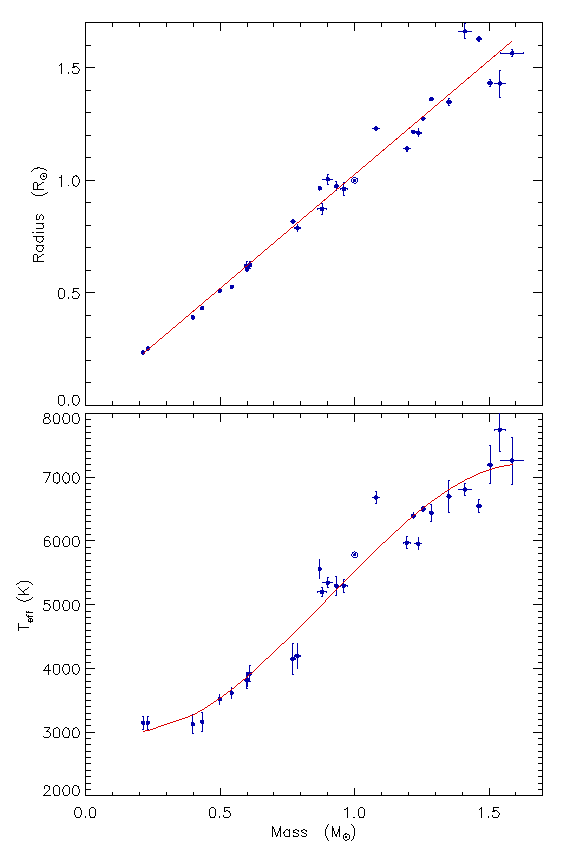
\includegraphics{3-images/final-EB.eps}
    \caption{Mass--radius and mass--$T_{\rm eff}$\ diagrams for exoplanet host stars. The filled circles show the properties of stars in eclipsing binary systems and the Sun is represented by a $\odot$. The solid lines represent the mass--radius and mass--$T_{\rm eff}$\ relations. Image take from \protect\citet{2009MNRAS.394..272S}.}
    \label{introduction:fig:TEPcalibration}
\end{figure}


Testing evolutionary models requires a diligent comparison of mass, radius and temperature measurements. Because there is a commonly observed discrepancy between between observed and predicted fundamental parameters (Sect. \ref{introduction:tension}), it is common-place to derive empirical relations instead. A rudimentary approach by \citet{2009MNRAS.394..272S} achieved this using a sample of 29 stars in eclipsing binaries (plus the Sun) which covers the masses $0.124$-$1.586\,M_\odot$  (Fig. \ref{introduction:fig:TEPcalibration}). They fitted a first-order polynomial to the mass-radius relation which did not account for [Fe/H] and age,
%
\begin{equation}
    R_\star = (0.00676 \pm 0.03408) + (1.01824 \pm 0.03368) M_\star,
\end{equation}
%
where $R_\star$ and $M_\star$ are in solar units. The authors fit has an rms scatter of 0.073\,$R_\star$ about the fit; the scatter is significantly smaller for low-mass stars ($\leq 0.6\,M_\odot$) but there are less than 10 stars with masses below 0.6\,$M_\odot$. \citet{2009MNRAS.394..272S} also present an empirical mass-temperature relationship,
%
\begin{eqnarray}
T_{\rm eff} & = & (3217 \pm 564) - (2427 \pm 2304) \cdot M_\star \nonumber\\
      &   & + (7509 \pm 2802) \cdot M_\star^2 - (2771 \pm 1030) \cdot M_\star^3,
\end{eqnarray}
%
which has an rms scatter of 328\,K about the best fit. 


\begin{figure}
    \centering
    \includegraphics[width=\textwidth]{3-images/f9.pdf}
    \caption{Top: $R_*$ as a function of stellar $T_{\rm eff}$. The derived $R_*$ depends on $T_{\rm eff}$ so the errors are strongly correlated. A typical error is shown a gray ellipse in the top left of the plot. The best-fit ignoring [Fe/H] is shown as a dashed blue line. Bottom: residual from the best-fit. Points are coloured according to their metallicity. Image taken from \protect\citet{2015ApJ...804...64M}.}
    \label{intro:fig:Mann3}
\end{figure}


\begin{figure}
    \centering
    \includegraphics[width=\textwidth]{3-images/f4.pdf}
    \caption{Mass--radius diagram for stars in our sample (red circles) and those from low-mass eclipsing binaries (LMEBs, blue stars). A typical error bar on our measurements is shown to the left. Stars in our sample are color-coded by their metallicity. The fit to both samples is shown as a dashed line. The bottom panel shows the fractional residual between these two fits. Image taken from \protect\citet{2015ApJ...804...64M}.}
    \label{intro:fig:Mann4}
\end{figure}


Interferometry can provide both radius and temperature to a high precision. In addition to the luminosity relations stated above, \citet{2015ApJ...804...64M} created an empirical radius-temperature calibration (Fig. \ref{intro:fig:Mann3}),
%
\begin{equation}
    R_\star = \left( a + bX + cX^2 \right) \times (1 + f[Fe/H])
\end{equation}
%
where $X = T_{\rm eff} / 3500$\,K (Table \ref{intro:table:mann}). This calibration has a significant scatter in radius of 13\% which is reduced to 9\% when metallicity is accounted for.  Interformetric measurements are excluded from empirical mass relations as the mass of a single star is typically determined from its colours. \citet{2015ApJ...804...64M}, who determined stellar mass through colour relations from \citet{2000A&A...364..217D}, attempted to create a \textit{semi-empirical} mass-radius relation with a second order polynomial. Their fit is compared to a sample of detached eclipsing binaries with mass and radius errors below 5\% and find a notable discrepency above 0.65\,$M_\odot$. The authors state that model-inferred masses better reproduces the mass-luminosity relation measured for low-mass eclipsing binaries and thus the disagreement in Fig. \ref{intro:fig:Mann4} is most likely due to errors in the luminosity relation of \citet{2000A&A...364..217D}, which was based on only 3 objects with masses in this range.

\begin{figure*}[!htb]
\centering
\begin{minipage}{0.47\linewidth}
\includegraphics[angle=270,scale=0.45]{3-images/stellar_mass_as_teff_metal_harps_m_gto_v26feb15.png}
\end{minipage}
\begin{minipage}{0.47\linewidth}
\includegraphics[angle=270,scale=0.45]{3-images/stellar_radii_as_teff_metal_harps_m_gto_v26feb15.png}
\end{minipage}
\caption{Stellar mass (left panel), and radius (right panel), as a function of the effective temperature. Stars are plotted using different colours and symbols according to their metallicity. Several fits for fixed metallicity values are plotted: +0.15 (dashed line), +0.00 (solid line), -0.15 (dash-dotted line), and -0.30 (dotted line). The upper left panel shows the differences between the mass and those derived by using  \protect\cite{1993AJ....106..773H} relationship. Image taken from \protect\citet{2015A&A...577A.132M}.}
\label{intro:fig:mald}
\end{figure*}

Similar relations were derived by \citet{2015A&A...577A.132M} using interferometric observations of M-dwarfs. They fitted radii with masses calculated from the mass-luminosity relations of \citet{1993AJ....106..773H} using a second-order polynomial,
%
\begin{equation}
    R = 0.0753 + 0.7009 M + 0.2356M^2.
\end{equation}
%
There are significantly more calibrators in the \citet{2015A&A...577A.132M} sample than the \citet{2009MNRAS.394..272S} and provides a much tighter fit; the rms about the best fit is 0.02\,$M_\odot$ and 0.02\,$R_\odot$. However, there sample consists of stars measured by intereferometry and those in eclipsing binary systems and there is no attempt to account for age or metallicity. However, they do form mass-temperature and radius-temperature relations using third-order polynomials which account for metallicity,
%
\begin{eqnarray}
    M_\star &=& -171.616 + 0.139 T_{\rm eff} - 3.776 \times 10^{-5} T_{\rm eff}^2 \nonumber \\
    &+&3.419 \times 10^{-9} T_{\rm eff}^3 + 0.382 \rm [Fe/H];
\end{eqnarray}
\begin{eqnarray}
    R_\star &=& -159.857 + 0.130 T_{\rm eff} - 3.534 \times 10^{-5} T_{\rm eff}^2 \nonumber \\
    &+&3.208 \times 10^{-9} T_{\rm eff}^3 + 0.347 \rm [Fe/H].
\end{eqnarray}
%
These calibrations (Fig. \ref{intro:fig:mald}) are relatively good: the scatter in mass and radius is 0.02\,$M_\odot$ (13.1\%) and 0.02\,$R_\odot$ (11.8 \%) respectively and are valid for $3340 \, \rm K < T_{\rm eff} < 3840\, \rm K$ and $-0.4 \, \rm dex < \rm [Fe/H] < +0.16\, \rm dex $. The authors caution that relative errors in mass tend to increase for low-mass stars, and can be up to 40\% for stars with mass below 0.25\,$M_\odot$. The same is true for uncertainty in radius and can be larger than 20\% for stars with radius below 0.35\,$R_\odot$. A possible explanation for the increase in mass error for later-type M-dwarfs is that the relative mass errors from the \citet{1993AJ....106..773H} relationship tend to be larger at lower masses.


\section{Eclipsing binary, low mass}\label{introduction:EBLM}
% lack of calibratable points
% solution lies with EBLMs

Measuring the absolute parameters of M-dwarfs typically involves stars which are measured by interfereometry or those in binary configurations such that the companions occult the light from one another.  For low-mass stars ($< 0.6\,M_\odot$) there is a dearth of systems with absolute parameters known to the desired precision of a few percent. A recent compilation of M-dwarfs with masses and radii known to better than 10\% yield only 90 M-dwarfs \citep{2018arXiv180505841C}. The reason is due to the intrinsic brightness of M-dwarfs and low-probability of finding eclipsing binary systems from which mass and radius can be empirically derived. While the sample presented by  \citep{2018arXiv180505841C} is sizeable, it is not large enough to reliably determine empirical relations and they are not measured using consistent and homogenous techniques.

A solution to this problem is in the remit of exoplanet surveys. The Wide Angle Search for Planets  (WASP; \citealt{2006PASP..118.1407P})  is a survey for $0.8$--$ 2 \rm \, R_{Jup}$ objects transiting solar-like stars. Objects in this radius range can have masses which span three orders of magnitude, from Saturn-like planets to M-dwarfs. Consequently, WASP photometry has been used to identify hundreds of FGK stars with transiting M dwarf companions as a by-product of its successful exoplanet search. These systems are termed EBLMs (eclipsing binary, low-mass). The EBLM consortium has invested considerable effort to characterise these systems, including hundreds of hours of telescope time to measure their spectroscopic orbits. The determination of absolute parameters of EBLM systems has been coordinated within the EBLM project. This first three instalments of the project measured the absolute parameters of 4 EBLMs: EBLM I \citep{2013A&A...549A..18T}, EBLM II \citep{2014A&A...572A..50G} and EBLM III \citep{vonBoetticher2017}. Secondary eclipses of J0113+31 (EBLM II) resulted in an effective M-dwarf temperature that is $\sim600$\,K hotter than predicted with evolutionary models. The fourth instalment (EBLM IV) was the product of hundred of hours of observations of EBLMs leading to the spectroscopic orbits of 118 EBLM systems.  


%The accumaltion of this work has lead to the absolute parameters of 4 EBLM systems as part of the EBLM project (\citealt{2013A&A...549A..18T}, \citealt{2014A&A...572A..50G}, \citealt{vonBoetticher2017}, \citealt{Triaud2017}). 

%The main aim of the EBLM project is to improve our understanding of low-mass stars using accurate mass and radius measurements for transiting companions to FGK stars.

Almost a thousand candidate EBLM systems have been flagged as a result of the WASP project.%
\footnote{As of 10$^{th}$ Oct 2018.}
%
The M dwarfs in EBLM systems are most likely to be found around F stars as oppose to G-/Kstars. The reason for this has its origins in tidal evolution theory. If the rotation of the primary star is less than that of the companion stars orbital period, then the torque induced by tidal interaction will increase the rotation of the host star. However, this is at the expense of the semi-major axis which must decrease in order to conserve angular momentum. This causes a spiral-like orbit which may eventually lead to engulfment of the low-mass companion. This is most probable for G/K host stars whereas the rotation of F-type hosts is sufficient to avoid colliding (\citealt{2017IAUS..328..308P}; \citealt{2011A&A...525A..68B}; \citealt{2011A&A...533A..83B}).

The sample presented by \citet{Triaud2017} is ideal to measure the absolute parameters of M-dwarfs in EBLM systems. As they were discovered by the WASP project, they are in transiting configurations which provides information about the radii of each component. The light from the M-dwarf companion is significantly small such that it is only possible to measure the radial velocity for the brighter star. Subsequently, it is not possible to measure the absolute parameters without supplementary information from stellar models. The crux of the EBLM method (and perhaps its Achilles' heel) is how the mass and radius degeneracy is broken (see Sect. \ref{methods:eblmmass} for a discussion of different methods). The EBLM method hinges on the assumption that the uncertainties in evolutionary models for the primary star are much smaller than the absolute parameters which can be derived given the quality of the data. In reality, this may not be the case (see Sect. \ref{discuss:uncertainties}). 



 




\section{Motivation}

% context of exoplants
Over 200 planets have been found around M-dwarfs (\citealt{2013A&A...551A..48A}; \citealt{2014Sci...344..277Q}; \citealt{2014ApJ...784...45R}; \citealt{2015ApJ...800...99T}; \citealt{2015ApJ...804...10C}; \citealt{2015ApJ...809....7B}; \citealt{2016ApJ...818...87S}; \citealt{2016Natur.536..437A}; \citealt{2017Natur.542..456G}). These discoveries come from radial velocity surveys, transit surveys (both ground- and space-based) along with microlensing events. Of note are the discoveries of exoplanets around Trappist-1 \citep{2017Natur.542..456G} and Proxima Centauri \citep{2016Natur.536..437A} which increased the popularity of M-dwarfs for the public and scientists alike. 

M-dwarfs are promising targets for exoplanet surveys. At a given distance, $a$, from a star of radius $R_\star$, an exoplanet (of radius $R_p$) is less likely to transit an M-dwarf than a K-/F-dwarf as the transit probability scales as ∼ $R_\star /a$. Conversely, we find that exoplanets in habitable zones are more likely to transit an M-dwarf than a larger star due to $a$ decreasing faster than $R_\star$ as we consider less massive stars. The transit depth of an eclipse scales as $(R_p/R_\star)^2$ so a similar planet will produce a deeper eclipse for a lower-mass star. An M-dwarf's low luminosity results in a habitable zone which is much closer to the sun than solar-type stars. If finding exoplanets in the M-dwarf habitable zone is the goal, then there is an increased geometric probability of observing a transit as well as number of transits observed in a given time period \citep{2008PASP..120..317N}. Such systems are also suitable to study the atmospheres of exoplanets. \citet{2013Sci...342.1473D} showed that for a given planet of fixed mass, radius and equilibrium temperature, the signal-to-noise ratio of an exoplanet atmospheric spectral signature scales as $\sqrt{B_\lamda (T_\star)} / R_\star$, where $B_\lamda$ is the Planck function and $R_\star$ and $T_\star$ are the radius temperature of the M-dwarf. This ratio significantly increases for stars later than M2 meaning that fewer transit observations need to be co-added to significantly detect atmospheric features of an exoplanet that those found around solar-type stars. 

% speculoose
%   - Description
%   - Still need to determine the mas and radius of the host star
%   - Emprirical relations are OK but more absolute parameters a required totighten up the relations. 
One such project is the Search for habitable Planets EClipsing ULtra-cOOl Stars whos acronym was inspired by the sweet treat (SPECULOOS; \citealt{2018SPIE10700E..1ID}). Comprising of four 1-m telescope, it's mission is to detect terrestrial exoplanets around stars of spectral type M7 and later. SPECULOOS is designed to detect terrestrial exoplanets in the habitable zone of the nearest 500 red-/brown-dwarfs. This project should detect a few dozens of planets
%
\footnote{www.speculoos.uliege.be/cms/c_3272723/en/speculoos-exoplanets}
%
which will be seminal to our understanding of other worlds. A similar project is the MEarth project \citep{2010ApJ...718.1353I} which uses 16 0.4-m telescopes across two sites: 8 at Mount Hopkins, Arizona and 8 at the Cerro Tololo Inter-American Observatory, Chile. The atmospheres of exoplanets discovered from these surveys can be studied by the next generation of telescopes such as the 6.5-m James Webb Space Telescope (JWST; \citealt{2006SSRv..123..485G}) or the 24.5-m Giant Magellan Telescope \citep{2014SPIE.9145E..1CB}. However, a big question-mark remains for the reliability of stellar models for M-dwarfs, which ultimately control govern the precision of exoplanet properties. Thus, the need for reliable empirical calibrations of M-dwarfs are required to compliment stellar models. 

Empirical and semi-empirical relations presented in Sect. \ref{intro:empirical} do a moderately good job of linking fundamental parameters of M-dwarfs. There is, however, an significant scatter in these relations which may be a result of the intrinsic properties of M-dwarfs. It is clear that a larger sample of M-dwarfs with well-understood absolute parameters are required to derive better-understood empirical relations. To this end, I will measure the absolute parameters of 9 M-dwarfs in EBLM systems. Before I could achieve this, I had to find a fast and robust way to measure the stellar atmospheric parameters of the brighter star from a spectrum. I decided to use wavelet decomposition to achieve this task and inspired the first research question of this work: \\

\textbf{How well can we measure the atmospheric parameters of FGK stars using wavelet decomposition?}

Exoplanet candidates discovered by the WASP survey \citep{2006PASP..118.1407P} were typically observed with the CORALIE \'{e}chelle spectrograph \citep{2001Msngr.105....1Q}. CORALIE is optimised for radial velocity measurements, and raw spectra have significant systematic trends from \'{e}chelle merging and poor blaze-function corrections. Atmospheric parameters are usually measured by experienced spectroscopists using measurements of equivalent widths (e.g. \citealt{2013A&A...556A.150S}; \citealt{2014A&A...562A..10C}; \citealt{2015A&A...577A..67S}), synthetic models (e.g. \citealt{2016ascl.soft05004M}; \citealt{2012ascl.soft05004P}; \citealt{2017A&A...597A..16P}) or a combination of both (e.g. \citealt{2007MNRAS.379..773S}; \citealt{Doyle2015}). This is time consuming and a fast, reliable method to measure atmospheric parameters from CORALIE spectra was required.

This problem can be solved with wavelet decomposition. A wavelet is a special function in space which can identify noise and systematic trends when convolved with a stellar spectrum (see Sect. \ref{wavelet:wavelet_decomposition}). This was used to create an Bayesian method to measure $T_{\rm eff}$, [Fe/H], $V \sin i$ and $\log g$ for the primary star. These parameters inform  limb-darkening coefficients and the stellar models used to determine the masses, radii and age of EBLM systems. This leads to the second research question:\\

\textbf{To what extent can EBLM systems contribute to empirical mass-radius relationships at the bottom of the main sequence? }

Measurements of the absolute parameters of M-dwarfs from the sample of 118 EBLMs presented by \citet{Triaud2017} will almost double the current sample of M-dwarfs from the literature with masses and radii known to better than 10\% (assuming absolute parameters can be measured to a few percent and that some fraction are unsuitable). These measurements will test stellar models at the bottom of the main-sequence and allow reliable empirical measurements to be derived. 

However, it is growing increase evident that there are systemic uncertainties in the accuracy of different analysis techniques. Measurements of individual systems by different groups have lead to absolute parameters that differ by more than 10\% in some cases (e.g., \citealt{2013MNRAS.429...85C} vs \citealt{2017A&A...600A..55I} vs \citealt{2017AJ....154..100H}; or \citealt{2017ApJ...845...72K} vs \citealt{2017ApJ...849...11G}). Due to the dearth of M-dwarfs with reliable measurements, empirical relations are typically composed of results from different analysis methods making it difficult to interpret the observed scatter as astrophysical or methodological. The exoplanet community has faced a similar issue which lead to a community-wide data challenge. For example, the eclipse depths of exoplanet XO-3b observed with post-cryogenic Spitzer was measured by 7 different groups to assess the accuracy of each technique. This helped clarify the difference between instrumental and other sources of error \citep{2016AJ....152...44I}. In the absence of a data-challenge for EBLMs, I must assess the validity of my methods to determine possible sources of non-astrophysical scatter in future empirical relations derived from EBLMs.  





%The second part of the thesis stems from the first. We had a robust method to measure the atmospheric parameters F-/G-stars which have M-dwarf companions (EBLMs) that have been discovered by WASP. These systems provide an unique way to calibrate empirical mass-radius relations for the lowest-mass stars. To this end, Significant CORALIE telescope time has been invested to obtain spectroscopic orbits of EBLMs which constrains the systems mass ratio and eccentricity. With followup transit photometry from ground-/spaced-based instruments and accurate atmospheric parameters, we can accurately measure the masses, radii and age of EBLM systems. Such measurements are then used to test evolutionary models for the bottom end of the main sequence where deviations are routinely observed (e.g. \citealt{2014ApJ...797...31T}; \citealt{2015A&A...577A..42B}; \citealt{2017ApJ...844..134L}). 

%Measuring the masses,radii and age of EBLM systems is only half the story. Little consideration is given to factors which often ignored during the fitting procedure: how the degeneracy between the masses and radii are broken? Which evolutionary models are used? How is eccentricity treated? How are M-dwarfs compared to evolutionary models? With the succesfull launch of transiting exoplanet survey satellite (TESS; \citealt{2015JATIS...1a4003R}) and CHEOPS on the horizon \citep{2013EPJWC..4703005B} it is imperative to identify what needs to be done to develop techniques which feed into empirical calibrations. We also need to know how many EBLMs will have to be studied 



















































































\iffalse
\section{Exoplanets and habitability}

M-dwarfs are promising targets for exoplanet surveys. At a given distance, $a$, from a star of radius $R_\star$, an exoplanet (of radius $R_p$) is less likely to transit an M-dwarf than a K-/F-dwarf as the transit probability scales as ∼ $R_\star /a$. Conversely, we find that exoplanets in habitable zones are more likely to transit an M-dwarf than a larger star due to $a$ decreasing faster than $R_\star$ as we consider less massive stars. The transit depth of an eclipse scales as $(R_p/R_\star)^2$ so a similar planet will produce a deeper eclipse for a lower-mass star. An M-dwarf's low luminosity results in a habitable zone which is much closer to the sun than solar-type stars. If finding exoplanets in the M-dwarf habitable zone is the goal, then there is an increased geometric probability of observing a transit as well as number of transits observed in a given time period \citep{2008PASP..120..317N}. 

Over the past decades there has been major progress in finding exoplanets around M-dwarfs. Over 200 planets have been found around M-dwarfs (\citealt{2013A&A...551A..48A}, \citealt{2014Sci...344..277Q}, \citealt{2014ApJ...784...45R}, \citealt{2015ApJ...800...99T}, \citealt{2015ApJ...804...10C}, \citealt{2015ApJ...809....7B}, \citealt{2016ApJ...818...87S}, \citealt{2016Natur.536..437A}, \citealt{2017Natur.542..456G}). These discoveries come from radial velocity surveys, transit surveys (both ground- and space-based) along with microlensing. Of note are the discoveries of exoplanets around Trappist-1 \citep{2017Natur.542..456G} and Proxima Centauri \citep{2016Natur.536..437A} which has increased the popularity of M-dwarfs for the public and scientists alike. 

There have been recent advances in theoretical research along with observational evidence to support the conclusion that a myriad of other factors may disrupt the traditional idea of M-dwarf habitability (instead of just a function of $a$). The intense stellar activity of an early-life M-dwarf can lead to significant alterations in atmospheric chemistry \citep{2016PhR...663....1S}. In particular, the abundances of ozone \citep{2010AsBio..10..751S}, surface water,  molecular oxygen \citep{2015AsBio..15..119L} and CO$_2$ \citep{2015ApJ...806..249G} can be modified by stellar activity. In cases where close-in planets form with thick H$_2$ envelopes, however, stellar activity could photoevaporate these envelopes unveiling habitable cores \citep{2015AsBio..15..119L}.  

M-dwarf emission is stronger in the IR and near-IR and so gases that absorb there are expected to have an important contribution to the discussion of habitability. Molecules like CO$_2$, H$_2$O, CHG$_4$ and O$_3$ are able to absorb a larger fraction of flux from an M-dwarf compared to the same planet around a hotter star. Planets with dense CO$_2$ atmospheres could see an increase in surface habitability through increased surface temperature \citep{2011mamo.conf..447W}. However, at the distant end of the habitable zone the effects of Rayleigh scattering will supersede atmospheric warming by CO$_2$ leading to frozen surface conditions \citep{2016PhR...663....1S}.

The exoplanet GJ1214b is a super-earth transiting an M dwarf \citep{2009Natur.462..891C}. The importance of such a system is that it was first to have spectral observations throughout transit (\textit{transit spectroscopy}). This allowed for transit depth to be measured as a function of wavelength which, which is a proxy for the effective radius of the star. The ability to detect such variations depends on the atmospheric scale height,
%
\begin{equation}\label{scale_height}
    H = \frac{k_b T_p}{g_p\mu},
\end{equation}
%
where $T_p$ is the mean atmospheric temperature of the planet (K) and $\mu$ is the mean molecular weight (Kg). Assuming each molecular/atomic species has its own scale height, the radii (transit depth) of an exoplanet will appear to change at wavelengths where the species in question absorbs. This can be compared to models to infer the composition of exoplanets  (\citealt{2012ApJ...747...35B}, \citealt{2011A&A...526A..12D}, \citealt{2013ApJ...765..127F},  \citealt{2014Natur.505...69K}).  This technique hinges on a strong contrast between the the star and planet (i.e. the transit depth can be measured with relatively high accuracy). The highest contrast is obtained for bright, nearby M-dwarfs with inflated hot-Jupiters. Using the near infrared spectrograph (NIRSpec) and the near-infrared imager and slitless spectrograph (NIRISS) onboard the James-Webb space telescope will revolutionise our idea of habitability by probing the chemical composition of thousands of exoplanet systems \citep{2017A&A...600A..10M}. 


\section{Absolute parameters}

Determining the absolute parameters (mass, radius, age, luminosity, temperature) is no easy feat, yet it is imperative to understanding the interior workings of M-dwarfs. Such measurements provide crucial tests to evolutionary models at the bottom of the main sequence which feed into our understanding of planets found around them. The frequently use quote "\textit{know thy planet, know thy star}" is pertinent for low-mass stars where significant deviations from models are observed (see Sect. \ref{mass_radius_section}). The curiosity to understand exoplanets around M-dwarfs has driven astronomers to derive empirical relationships between observable and absolute parameters (e.g. \citealt{2015ApJ...804...64M}). Empirical relations are derived using measurements of absolute parameters using different techniques\footnote{The sample used in \citet{2015ApJ...804...64M} calculates mass from the empirical mass-luminosity relations of \citet{2000A&A...364..217D} and radius from surface temperature, trigonometric parallax and bolometric luminosity.}. In the following sections we describe a few of these. 

    \subsection{Interferometry and astrometry}
    
      \begin{figure}
    \includegraphics[width=\textwidth]{3-images/interferometer_basic}
    \caption{Basics of interferometry. Image taken from http://www.chara.gsu.edu.}
    \label{fig:interferometry_basics}
    \end{figure}
    
    \begin{figure}
    \includegraphics[width=\textwidth]{3-images/vis_diam}
    \caption{The normalised visibility amplitude for a star with angular diameter of 1 mas (blue) and 3 mas (red). Image taken from http://www.chara.gsu.edu.}
    \label{interferometry_visibility}
    \end{figure}
    
    
    \begin{figure}
    \includegraphics[width=\textwidth]{3-images/vis_binary}
    \caption{The normalised visibility amplitude for a binary system. The distance between peaks (blue arrow) provides an estimate of binary separation and the minimum visibility (purple line) is an estimate of flux ratio between the two stars. Image taken from http://www.chara.gsu.edu.}
    \label{fig:interferometry_binary}
    \end{figure}
    
    The light from a bright M-dwarf may be monitored simultaneously through two or more telescopes. The light from these instruments are combined to produce an interference pattern of alternating light and dark bands (\textit{fringes}; see Fig. \ref{fig:interferometry_basics}). The most common measurement in optical and infrared interferometry is a measurement of the amplitude of the fringes. This fringe contrast is often called the "\textit{visibility}" of the fringes.  The normalized visibility amplitude ($V$) is computed from the maximum and minimum intensity ($P$) of the fringes, given by
    \begin{equation}
    V = \frac{P_{max} - P_{min}}{P_{max} + P_{min}}.
    \end{equation}
    An unresolved point source will have a normalized visibility amplitude of 1.  For a spatially resolved star, light from across the stellar surface combines incoherently causing a drop in the visibility amplitude, making the normalized visibility amplitude less than 1 (Fig. \ref{interferometry_visibility}).  The bigger the star, the smaller the fringes and lower the fringe amplitude.  By measuring this drop in the fringe amplitude it is possible to measure the size, shape, and surface features of an M-dwarf. A binary star will produce two fringe packets, one for each star in the system.  If the separation between the stars is small enough, the fringe packets from each star will overlap, producing a periodic signal in the visibility amplitudes.  An example visibility curve for a binary star is shown in Fig. \ref{fig:interferometry_binary}.  The separation between the peaks in the visibility curve provides a measurement of the binary separation while the minimum visibility reflects the flux ratio between the components. 
    
    There have been many successful attempts to measure the radius and temperature of single field M-dwarfs (e.g. \citealt{1997A&A...325..159L}, \citealt{2006ApJ...644..475B}, \citealt{2001AAS...198.5120N}, \citealt{2003A&A...397L...5S}; \citealt{2009A&A...505..205D},  \citealt{2012ApJ...757..112B}; \citealt{2015csss...18..839V}). The fraction of M-dwarfs which have companions within 1000\,AU is estimated to be 40\% (\citealt{1992ApJ...396..178F}, \citealt{2006ApJ...640L..63L}, \citealt{2010ApJS..190....1R}); The majority of these binaries have separation above 5" from the  (50\,AU; \citealt{2015ApJ...804...64M}). Interferometry can monitor the relative positions of each component $\Delta \alpha$, $\Delta \delta$) relative to the centre of mass. An example is given by \citet{2016AJ....152..141B} who used white-light interferometric observations from the Hubble Space Telescope with radial velocity data from the McDonald Observatory to obtain astrometric solutions of M-dwarfs in binary systems. They achieved mass uncertainties as low as 0.4\% in some cases (median error of 1.8\%), but little insight regarding the radii of each component. \citet{2012ApJ...757..112B} acquired interferometric observations at the CHARA Array in the near-infrared $K'$ and $H$ bands \citep{2005ApJ...628..453T} for 21 nearby, single and bright red dwarfs. They measured radii with an uncertainty below 3\% and uncertainty in $T_{\rm eff}$ below 1\% and robustly demonstrate that models over-predict $T_{\rm eff}$ by $\sim3\%$, and under-predict radii by $\sim5\%$. Obtaining the mass for single stars often requires photometric calibrations for red-dwarfs (e.g. \citealt{1993AJ....106..773H}, \citealt{2000A&A...364..217D}). The  uncertainty associated with these relations can be up to $10\,\%$ which makes it difficult to test evolutionary models. 
    %greatly exceeds uncertainties in radii quoted in \citet{2016AJ....152..141B}; this makes it challenging to assess radius inflation for single stars observed with interferometry (see Sect. \ref{mass_radius_section}) .
    
    
    \subsection{Eclipsing binary systems}
    
The geometrical configuration of equal mass M-dwarf binaries is such that one star passes in front of the other diminishing some of the light. Because M+M dwarf binaries will have a similar luminosity ratio, it is possible to measure the drop in flux as each star passes in front of the other. This sets the scale of radii for each component. Another consequence of equal luminosity is is that spectral features from each M-dwarf can be identified in (often) unresolved spectra. This may permit a measurement of temperature and radial velocity for each star from a single spectrum. Radial velocity measurements for each star set the mass scale of the system. Eclipsing binaries where both spectra are discernible are called double-lined eclipsing binaries (DEBs). In John Southworth's catalogue of double-lined eclipsing binaries \citep{2015ASPC..496..164S} there are 11 systems in which both systems have the M-spectral type (\citealt{2010ApJ...712.1003W}, \citealt{2002ApJ...567.1140T}, \citealt{2011ApJ...728...48K}, \citealt{2018AJ....155..114H}, \citealt{2003A&A...398..239R}, \citealt{2017ApJ...845...72K}, \citealt{2011ApJ...742..123I}, \citealt{2016ApJ...816...21D}, \citealt{2016ApJ...816...21D}). 



\begin{figure}
    \centering
    \includegraphics[scale=0.6]{3-images/WD+M.png}
    \caption{Model fits to the ULTRACAM light curves of NN Serpentis with residuals shown below. Top: Full orbital phase. Centre: Around the primary eclipse. Bottom: Around the secondary eclipse. Finer binning was used around both the eclipses. The r’ light curves are slightly noisier around the eclipses because there is no VLT photometry for that filter. The secondary eclipse light curves are also shown with a model with the secondary eclipse turned off. Points around the primary and secondary eclipses were given twice the weighting of other points resulting in some residual effects seen in the residuals. Image taken from \protect\citet{2010MNRAS.402.2591P}}
    \label{fig:WD_M_binary}
\end{figure}



A different approach is to measure eclipsing binary systems where only one of the stars is an M-dwarf. One such example is M+ white-dwarf systems (M+WD). The small size of the M-dwarf ($R \sim 1\,R_\oplus$) results in very sharp, total eclipses which can be used to measure radii to a precision of a few percent (Fig. \ref{fig:WD_M_binary}; \citealt{2010MNRAS.402.2591P}). Consequently, it is possible to obtain a clean M-dwarf spectrum free from contamination of the white dwarf from which atmospheric parameters can be derived. The cooling of white dwarfs is also well understood (e.g. \citealt{1997ApJ...486..413S}, \citealt{2013A&A...555A..96S}, \citealt{2014Natur.515...88V}) making them ideal systems to determine the age of an M-dwarf. 

In cases where no secondary eclipse are observed (WD eclipsing the M-dwarf) there is a degeneracy between the scaled radii $R_{WD}/a$, $R_{M}/a$ and inclination ($i$). For these systems an additional piece of information is required such as 1) the rotational broadening of the M-dwarf and/or 2) the gravitational red shift of the white dwarf \citep{2010MNRAS.402.2591P}.  These systems have experienced a brief common envelope phase when the progenitor star to the white dwarf evolved off the main sequence. This has a negligible effect on the low-mass star as the common envelope phase is short (0.001-0.01\,Myr) compared to the thermal timescale of the M-dwarf (0.1-1\,Gyr). Additionally, the common envelope has a much higher specific entropy than the surface of an M-dwarf so very little accretion will take place \citep{1991ApJ...370..709H}.
    
    


\section{Mass and radius}\label{mass_radius_section}



\section{Eclipsing binary, low mass}

The Wide Angle Search for Planets  (WASP; \citealt{2006PASP..118.1407P})  is a survey for $0.8$--$ 2 \rm \, R_{Jup}$ objects transiting solar-like stars. Objects in this radius range can have masses which span three orders of magnitude, from Saturn-like planets to M-dwarfs. Consequently, WASP photometry has been used to identify hundreds of FGK stars with transiting M dwarf companions as a by-product of its successful exoplanet search. These systems are termed EBLMs (eclipsing binary, low-mass). We have invested considerable effort to characterise these systems, including hundreds of hours of telescope time to measure their spectroscopic orbits. The main aim of the EBLM project is to improve our understanding of low-mass stars using accurate mass and radius measurements for transiting companions to FGK stars (\citealt{2013A&A...549A..18T}, \citealt{2014A&A...572A..50G}, \citealt{vonBoetticher2017}, \citealt{Triaud2017}).

The large number of EBLMs provides a healthy sample of absolute parameters for M-dwarfs using methods akin to exoplanet research. Most of the M dwarfs discovered in binary systems with main sequence stars are typically F+M binaries as oppose to G-/K-M binaries. The reason for this has its origins in tidal evolution theory. If the rotation of the primary star is less than that of the companion stars orbital period, then the torque induced by tidal interaction will increase the rotation of the host star. However, this is at the expense of the semi-major axis which must decrease in order to conserve angular momentum. This causes a spiral-like orbit which may eventually lead to engulfment of the low-mass companion.  This is most probable for G/K host stars whereas the rotation of F-type hosts is sufficient to avoid colliding (\citealt{2017IAUS..328..308P}, \citealt{2011A&A...525A..68B}, \citealt{2011A&A...533A..83B}). 

\section{Motivation for this work}

From an exoplanet perspective, the fundamental properties of M-dwarfs constitute the bedrock from which the accuracy and reliability of exoplanet parameters are conceived. It is not until we step back and take a macro perspective that we observe our bedrock is far from level. This challenges our idea of exoplanets found around M-dwarfs, the IMF for low-mass stars, young star clusters and proto-planet disk properties \citep{2013ApJ...771..129A}.

Measurements of M-dwarfs from interfereomtry and eclipsing binary systems are beginning to test the finer details of stellar models. Eeach method contributes to the study of low mass stars and they both paint the same picture: \textit{some M-dwarfs are inflated, but not all}. The exact reason for this is unclear. One can also question the reliability/accuracy of pipelines used to measure eclipsing binary systems. For example, measurements of fundamental stellar parameters by different groups differ by up to 10\% in the case of T-Cyg1-12664 (\citealt{2013MNRAS.429...85C} VS \citealt{2017A&A...600A..55I} VS \citealt{2017AJ....154..100H}) and PTFEB132.707+19.810  (\citealt{2017ApJ...845...72K} VS \citealt{2017ApJ...849...11G}). The field is afflicted by a crisis of repeatability. 

\begin{sidewaysfigure}[ht]
    \includegraphics[width=\textwidth]{3-images/EBLM_flow-Page-1.png}
    \caption{Generalised flow chart used for this work.}
    \label{fig:EBLM_flow_chart}
\end{sidewaysfigure}

In this work we measure the absolute parameters of M-dwarfs in EBLM systems. They are discovered in abundance as a by-product of WASP and have been followed spectroscopy and photometry. This provides crucial radial velocity measurements to determine the mass of both components as well as atmospheric parameters of the primary star. We jointly fit radial velocity measurements and light curves from a suite of ground-/space-based instruments to determine a best-fitting orbital solution. We break the mass degeneracy by interpolating evolutionary models to estimate the mass and age of the primary star, and thus the mass of the M-dwarf companion. The modus operandi for this work is summarised in Fig. \ref{fig:EBLM_flow_chart}. From these measurements I will attempt to answer the following questions:

\begin{enumerate}
    \item Is it possible to measure accurate atmospheric parameters for noisy spectra in which the primary objective is radial velocity measurements?
    
    \item How accurately and precisely can we measure the masses, radii and age of EBLMs?
    
    \item Do EBLMs show the same radius problem observed elsewhere in the literature? 
    
    \item Is the radius problem correlated with observable parameters? 
\end{enumerate}

\fi










%Main Motivation Program Data Challenge
 
 

%Why EBs, and Why Now?

 
%The fundamental properties of stars constitute a bedrock upon which much of modern astrophysics is built. It is a maxim of stellar astrophysics that the properties and lifecycle of a star are largely set by its mass, and hence it is crucial to calibrate the mass predictions of models. Uncertainties in model-derived properties constitute the dominant systematic error for in-situ measurements of the IMF (Bastian et al. 2010), determinations of star cluster ages (e.g., Pecaut et al. 2012), and comparison of protoplanetary disk properties to those of mature planetary systems (Andrews et al. 2013). Stellar models are also crucial for interpreting exoplanet discoveries via all methods, whether from model-dependent masses (for RVs), radii (for transits), or ages (for direct imaging). The gold standard for benchmarking stellar evolutionary models is to use double-lined eclipsing binaries, for which it should be possible to simultaneously derive model-independent masses, radii, temperatures, and luminosities.



%Eclipsing binary studies are now testing the detailed astrophysics of stellar evolutionary models (e.g., Stassun et al. 2014; Feiden 2016). Analyses can routinely achieve precisions of 1-3% with robust analysis of high-quality datasets, and have enabled a mapping of the stellar mass-radius relation to as low as 0.1 Msun (e.g., Torres et al. 2010), while also revealing potential scatter in the relation of 5-10\% or more in some mass ranges. In particular, these studies suggest that models could under-predict stellar parameters because they don't fully capture rotation/activity (e.g., Lopez-Morales 2007; Kraus et al. 2011). The wide-field, synoptic monitoring of K2 has also vastly expanded the number of eclipsing systems in young, pre-main-sequence populations, previously limited to a modest number that sparsely sampled parameter space (e.g., Stassun et al. 2006; Gillen et al. 2014) enabling calibration of stars' contraction onto the main sequence. These studies have indicated substantial disagreements between observations and models for the masses, radii, temperatures, and luminosities of stars, and hence also for model-derived parameters like ages (e.g., Kraus et al. 2015, 2017; David et al. 2015; 2016; Gillen et al. 2017).



%However, it is growing increasingly evident that there are large systematic uncertainties in the accuracy of the analysis techniques used to measure those stellar properties for eclipsing binary systems. Analyses of individual systems by different groups have led to stellar parameters that differ by tens of percent (e.g., Cakirli et al. (2013) vs Iglesias-Marzoa et al. (2017) vs Han et al. (2017); or Kraus et al. (2017) vs Gillen et al. (2017)). Due to the rarity of eclipsing systems and the individual discovery of most EBs, the mass-radius relations constructed to date have effectively been based on as many different pipelines and types of datasets as there are systems. These pipelines can differ fundamentally from each other. For example, some authors model the occulted stellar surfaces with empirical polygonal surface brightness distributions, such as Wilson & Devinney (1971) or the PHOEBE code of Prsa et al. (2016), while others use approximations that allow analytic solutions, such as the JKTEBOP code of Southworth et al. (2004) or Kraus et al. (2015). It is therefore extremely difficult to know if the observed scatter results from astrophysics or from the analysis methods, or even if the mean sequence needs to shift due to non-Gaussian distribution of systematic pipeline uncertainties. Our field is currently limited by a crisis of repeatability.



%Exoplanet science has struggled with similar obstacles, particularly in the interpretation of transiting exoplanet data, and we can look to the transit community for a potential solution: a community-wide “data challenge” (e.g., Ingalls et al. 2016). Such challenges are structured to provide all groups with uniform, high-quality datasets that test different regimes of parameter space, and then provide those groups with a forum to present their analysis and results; the comparison of all these results then offers an empirical calibration of the expected scatter, while detailed comparison of offsets can also point toward desirable methodological design choices. As we describe further below, an “eclipsing binary data challenge” would ideally consist of both real datasets (both published and unpublished), as well as synthetic datasets that are produced by each group (by inverting their pipelines) and then distributed to all other groups. This choice would preserve double-blindness and place all groups on an equal footing. We anticipate that the results could easily be summarized in a refereed journal article, as Ingalls et al. (2016) did.



%We are organizing a dual-purpose splinter session at Cool Stars 20, which will simultaneously present and challenge the state-of-the-art results emerging from this fields. Our splinter will provide a venue for the leading teams in EB studies to present their newest scientific results, often inspired by cutting-edge observations from Kepler/K2/TESS and from the newest generations of ground-based spectrographs. However, we will also organize a data challenge (occurring before and during the meeting) wherein each participating team must analyze uniform, high-volume datasets that we hope (but do not expect) would yield consistent answers across all the teams who are currently pushing the forefront in stellar astrophysics.



%This splinter session is very timely, given the ongoing renaissance of stellar variability studies to emerge from Kepler, K2, and soon TESS, combined with the revolutionary advances in distance (and hence luminosity) measurements from Gaia DR2. Across broad swaths of stellar parameter space, these missions will expand the number of calibrators from a few sparse examples into the hundreds or even thousands, ending the era of Poisson-limited stellar characterization and ushering in the era of systematics-limited stellar astrophysics. Our splinter session is aimed squarely at understanding and minimizing those systematic uncertainties, unleashing the full power of these revolutionary space telescopes.



%REFERENCES

%Andrews, S. et al. 2013, ApJ, 771, 129

%Bastian, N. et al. 2010, ARA\&A, 48, 339

%Cakirli, O. et al. 2013, MNRAS, 429, 85

%David, T. et al. 2015, ApJ, 814, 62

%David, T. et al. 2016, ApJ, 816, 21

%Feiden, G. 2016, A\&A, 593, 99

%Gillen, E. et al. 2014, A\&A, 562, A50

%Gillen, E. et al. 2017, ApJ, 849, 11

%Han, E. et al. 2017, AJ, 154, 100

%Iglesias-Marzoa, R. et al. 2017, A\&A, 600, A55

%Ingalls, J. et al. 2016, AJ, 152, 44

%Kraus, A. et al. 2011, ApJ, 728, 48

%Kraus, A. et al. 2015, ApJ, 807, 3

%Kraus, A. et al. 2017, ApJ, 845, 72

%Lopez-Morales, M. 2007, ApJ, 660, 732

%Pecaut, M. et al. 2012, ApJ, 746, 154

%Stassun, K. et al. 2006, Nature, 440, 311

%Stassun, K. et al. 2014, NewAstRev, 60, 1

%Torres, G. et al. 2010, A\&A Rev, 18, 67

 
 

% Things to note
%	-----------------------------------------
%				PARAGRAPH 1
%	-----------------------------------------
%
%	- leads to higher spot coverage & supression of convections
%	- Magnetic field strength and magnetic activity have long been known to be coupled to rotation (Parker 1955)
%	- recent observations affirm that M dwarf stars with rotation periods less than ∼5 days all show evidence of magnetic activity through chromospheric emission (e.g., West et al. 2015; Newton et al. 2017).
%	- EBs are preferentially inflated because of observational biases:  they tend to have short orbital periods (P < 5 d)
%	- Kraus et al. (2011) have suggested adding a rotation parameter into Mass−Radius relations for M dwarf stars
%	- A large fraction of single M dwarf stars are also found to be rapid rotators (more than one third of the mid-to-late M dwarf stars in the MEarth survey have rotational periods less than one day;  Newton et al. (2016))
%	- Can't compare EB radii to Interferometry radii because the Interferometry sample for FAST rotators is too small (Proxima Centauri and Barnard’s Star; Boyajian et al. 2012) have rotation periods around 80-130 days (Benedict et al. 1998).
%	-----------------------------------------
%				PARAGRAPH 2
%	-----------------------------------------
%
% 	- Could just be an effect of EB
%	- Disk disruption and/or tidal effects from close binaries could alter the evolutionary history of EBs such that rotation is not the key factor responsible for the larger-than-expected radii (Meibom et al. 2006; Morgan et al. 2012)
%	- Magnetic cool spots on active M dwarf stars are preferentially distributed near the poles (Morales et al. 2010 ; as seen by Granzer et al. 2000; Jeffers et al. 2007; Strassmeier 2009).
%	- therefore the radii could be overestimated by up to 6% by parameter extraction codes that assume circular stellar disks when modelling EB light curves.
%	- Also, reanalysis of EB data from multiple groups has oftentimes lead to vastly different stellar parameters, calling into question the accuracy of parameters extracted from EBs (Han et al. 2017).
%	-----------------------------------------
%				PARAGRAPH 3
%	-----------------------------------------
%	- Two scenarios on how B fields lead to inflated radii
%	- (1) strong magnetic fields inhibit convective flows (modeled by decreasing the mixing length parameter)
%	- (2) large magnetic cool spots decrease the overall effective temperature of the star, and thus increase the radius since the luminosity is unchanged.
%	- Only stars above the fully convective boundary would be affected by scenario (1), because their interiors are nearly adiabatic and decreasing the mixing length parameter has little effect (Chabrier et al. (2007)).
%	- Chabrier et al. (2007) also showed that scenario (2) alone could inflate the radii of M dwarf stars seen in EBs, but only with a large spot covering fraction of 30-50% of the stellar surface.
%	- Feiden & Chaboyer (2014) used the Dartmouth Magnetic Stellar Evolution Tracks and Relations (DMSETR; Feiden & Chaboyer 2012) to explore both of these scenarios:
%		- Instead of modeling scenario (1) using a decreased mixing length parameter, they modeled how the magnetic field could stabilize convection, and found that it could inflate the radii of fully convective stars by 5-6% if extremely strong interior magnetic fields were invoked (40 MG).
%		- However, theoretical predictions of interior field strength concluded that the above-quoted field strengths are unreasonably large (Browning et al. 2016). On the other hand, MacDonald & Mullan (2017) used a similar approach to that of Feiden & Chaboyer (2014), but found interior magnetic fields strengths on the order of 10 kG could inflate the radii of fully convective stars to a similar degree as seen in EBs.





%
% 3. Lack of theoretical models and chemical constraints
%	- Spectra is hard to measure params from



% Things to note
%	-----------------------------------------
%				PARAGRAPH 1
%	-----------------------------------------
%
%	- Need a solid theoretical understanding of the fundamental parameters of low-mass stars
%	- Need precise sample of accurate and homogeneously measure 
%	- Need more interferometry measurements
%	- We have more EB measurements but we need projects like the EBLM project to get more homogenous measurements 
%	- There is no interferometric equivalent, but wide angle surveys (EBLM project) can find the closest and brightest ones to be followed up. 
%		- interferometry can get flux ratio to assess if Teff is probable or not
%		- Could also get physical separation if those had GAIA parallax measurements 
%	- But TESS will only be sensitive to the brightest and closest systems,  perfect for interferometry!
%	- TESS will download full-field images sampled every 30 minutes (Ricker & MORE 2009), allowing it to detect potentially habitable M-dwarf exoplanets over the whole sky down to around 14th magnitude.
%	-----------------------------------------
%				PARAGRAPH 2
%	-----------------------------------------
%
%	- Need a comprehensive assessment of method VS results to assess discrepancies from:
%		- Choice of Limb darkening 
%		- Choice of lightcurve model
%		- Method to get [Fe/H] and Teff  (colours, 
%		- Choice of evolutionary models (MLT He enhancement)
%			- OR colour mass relations  (which are naff but are out there)
%	- Draw parallels with the H&H exercise used in working group - quote results (get from person...)
%	-----------------------------------------
%				PARAGRAPH 3
%	-----------------------------------------
%	
%	- precise characterization of these objects from the available observables
%	- Calibrate the mass-radius-luminosity relation with extra parameters:
%		- Rotations, temperature, binary? 
%	- This will be valuable to quickly and accurately estimate the atmospheric parameters from past, and upcoming survey missions. 
%	- Talk about legacy missions: WASP, KELT, HATNET, MEARTH, etc. 
%	- Talk about importance for future missions: TESS, PLATO, SPECULOOS (semi on-line) 
%	-----------------------------------------
%				PARAGRAPH 4
%	-----------------------------------------
%	- To date, obtaining spectroscopy for every possible M-dwarf in the sky down to the relevant magnitudes for TESS (i.e. Gaia G≈14.5, I≈14) has been infeasible. No instrument has had the combination of a sufficiently wide-field (5-10° diameter field-of-view), aperture in the >1 m range, and multi-object spectroscopic capability for hundreds of objects across that wide-field.
%	- There are now two more instruments
%		- (1) FunnelWeb (Rains et al. 2018, in prep.) is is a multiobject stellar survey of the Southern Hemisphere set to commence observations in July 2018. It will cover the entire southern sky (excluding only the most crowded regions with δ ≤ 0°, |b| ≥ 10°) and obtain high-quality (S/N 100) optical spectra for some ∼ 1.8 million stars down to a magnitude of Gaia G=14.5, aiming for 99% completeness at the G=12.5 level. The survey is enabled by the TAIPAN instrument on the recently refurbished 1.2 m UK-Schmidt Telescope at Siding Spring Observatory, which is able to simultaneously robotically position 150 optical fibres (or “Starbugs”) within a 6°field of view. The instrument operates over the wavelength range 3700-8700˚A, and has a spectral resolution of R ≥ 2000. The main goals of the survey include a spectral library with detailed stellar parameters (including Teff, log(g), [Fe/H] and [α/Fe]), including stellar spectra for targets being observed by the TESS satellite, with M-dwarfs a particular focus.
%	- LAMOST (Chu & Cui 1996) in the northern hemisphere.

\iffalse
\begin{itemize}
% \item M dwarfs are 70\% of all stars Bochanski et al. 2010


% \item faint so few measurements of radii with interferometry ($\leq 20$ Segransan et al. 2003; Demory et al. 2009; Boyajian et al. 2012;von Braun et al. 2014). 


\item For binary stars raidii is inflated by as much as 10-15 \%, and average at 5\% (e.g., Torres \& Ribas 2002; Kraus et al. 2011;
Han et al. 2017)

\item Thee transition from Earth-like planets to
Neptune-like planets is believed to occur around 1.5RE (Rogers 2015)

\item If stellar radii are in error by up to 15%,
based on simulations of planet occurrence rates expected for TESS (Sullivan et al. 2015), a significant fraction of the future super-Earth sized planets expected to be discovered by TESS would in fact be mini-Neptunes.

\item 10 \% radii error = 30 \% density error (rocky or metal dominated.

\item Tess With a 30 day baseline for photometric
observations for most of the sky, the majority of
the discovered exoplanets in the habitable zone will be around M dwarf stars (Muirhead et al. 2017).
\item Several studies have proposed that the larger-than expected radii of M dwarf stars in EBs are a result of activity and enhanced magnetic fields (often around a few kiloGauss for M dwarf stars; Donati et al. 2006; LopezMorales 2007; Chabrier et al. 2007).

\item Magnetic field
strength and magnetic activity have long been known to
be coupled to rotation (Parker 1955)

\item recent observations affirm that M dwarf stars with rotation periods less than ∼5 days all show evidence of magnetic activity through chromospheric emission (e.g., West et al. 2015; Newton et al. 2017).

\item Kraus et al. (2011) have suggested adding a rotation parameter into Mass−Radius relations for M dwarf stars.

\item A large fraction of single M dwarf stars are also found to be rapid rotators. Newton et al. (2016) found that more than one third of the mid-to-late M dwarf stars in the MEarth survey have rotational periods less than one day.

\item If rotation-induced magnetic fields cause largerthan-expected radii in EBs, then a large number of single stars should also have larger-than-expected radii. 

\item As of now we do not have a sample of rapidly rotating single stars with precise radius measurements; the mid-to-late M dwarf stars for which interferometric radii measurements are available (Proxima Centauri and Barnard’s Star; Boyajian et al. 2012) have rotation periods around 80-130 days (Benedict et al. 1998).

\item Alternatively, the inflation may solely be an effect present in EBs. Disk disruption and/or tidal effects from close binaries could alter the evolutionary history of EBs such that rotation is not the key factor responsible for the larger-than-expected radii (Meibom et al. 2006; Morgan et al. 2012).

\item Morales et al. (2010) showed that if magnetic cool spots on active M dwarf stars are preferentially distributed near the poles (as seen by Granzer et al. 2000; Jeffers et al. 2007; Strassmeier 2009), the radii could be overestimated by up to 6\% by parameter extraction codes that assume circular stellar disks when modeling EB light curves.

\item Also, reanalysis of EB data from multiple groups has oftentimes lead to vastly different stellar parameters, calling into question the accuracy of parameters extracted from EBs (Han et al. 2017).

\item Chabrier et al. (2007) suggested two inflation mechanisms (1)  strong magnetic fields inhibit convective flows (modeled by decreasing the mixing length parameter) (2)  large magnetic cool spots decrease the overall effective temperature of the star, and thus increase the radius since the luminosity is unchanged.

\item Chabrier et al. (2007) predict that only stars above the fully convective boundary would be affected by scenario (1), because their interiors are nearly adiabatic and decreasing
the mixing length parameter has little effect.

\item (2) alone could inflate the radii of M dwarf stars seen in EBs, but only with a large spot covering fraction of 30-50\% of the stellar surface.

\item Feiden \& Chaboyer (2014) used the Dartmouth Magnetic Stellar Evolution Tracks and Relations (DMSETR; Feiden \& Chaboyer 2012) to explore both of these scenarios in more detail. Instead of modeling scenario (1) using a decreased mixing length parameter, they modeled how the magnetic field could stabilize convection, and found that it could inflate the radii of fully convective stars by 5-6\% if extremely strong interior magnetic fields were invoked (40 MG).

\item However, theoretical predictions of interior field strength concluded that the above-quoted field strengths are unreasonably large (Browning et al. 2016).

\item MacDonald \& Mullan (2017) used a similar approach to that of Feiden \& Chaboyer (2014), but found interior magnetic fields strengths on the order of 10 kG could inflate the radii of fully convective stars to a similar degree as seen in EBs.

\item  a sample of rapidly rotating, single, fully convective stars needs to be studied to determine the level of inflation present. Aurora Y et al 2017

\item taken from Y et al 2017. We find that all three predictions that involve stellar evolutionary models show ‘Strong’ to ‘Very Strong’ evidence that the observed M dwarf stars are larger than model radius estimates. The radii reported in both Newton et al. (2016) and Dittmann et al. (2014) show 2- to 3-sigma levels of discrepancy between the quoted radii and the measured radii (where the measured radii are on average 6 − 7\% larger than reported radii). However, when we use the newest empirical relations from Benedict et al. (2016) and Boyajian et al. (2012) we find that both of the odds ratios and the BIC cannot rule out the null hypothesis, that there is no inflation. Even though the maximum likelihood occurs for radii 5\% larger than the relations predict, the increase in total probability is not enough to overcome the penalty imposed by adding a free parameter.

\item Vsini from spot modulation on M dwarfs comes from spots preferbly located on  the poles. Vsini from spectroscopy comes from primarly equatiorial rotation. Using Kepler data of more than 10,000 stars, Reinhold \& Gizon (2015) showed that there is a relationship between the horizontal rotation shear and the rotation period, where stars with faster rotation periods exhibited smaller shears. A relationship between the differential rotation and the effective temperature was observed by Barnes et al. (2005), where stars with cooler effective temperatures were found to have less differential rotation.

\item There is evidence that M dwarf stars do not follow an exact Skumanich-like relation between the rotation period and age (Skumanich 1972), but instead a rotation period dichotemy exists (Newton et al. 2016).

\item  Fully convective M dwarf stars can continue to be magnetically active and retain rotation periods of less than 10 days up until 5 − 7Gyrs West et al. (2008), then it appears that they shed angular momentum and rapidly migrate to periods greater than ∼30 days (Newton et al. 2016). This makes precise gyrochonology very difficult for these stars, however it is well established that rapid rotators are on average younger than slow rotating M dwarfs (West et al. 2008, 2015). 

\item Further evidence that age is not the sole contributing factor of the observed inflation is given by comparison with rotation periods observed in young clusters such as Pleiades and NGC 2516. For mid-to-late M dwarfs neither of  these young (∼ 120 − 150 Myrs) clusters are observed to contain stars with rotation periods longer than about 1.5 to 2 days (Scholz et al. 2011; Rebull et al. 2016a,b),

\item In a study of the metallicity of the MEarth sample (Newton et al. 2014), the average metallicity of the rapidly rotating stars is 0.14 ± 0.1dex. Therefore in our analysis we assumed a metallicity of 0.14 dex when comparing to isochrones. We find that by using a solar metallicity isochrone the average inflation can change by 1 − 1.5\%. Since this change in metallicity is more than one standard deviation and it can only account for a small amount of the observed inflation, this leads us to conclude that metallicity alone cannot be responsible for the inflation observed in our stellar sample. We note that the metallicities were measured using methods that may in fact be probing the carbon-to-oxygen ratios of the stars, and not the metallicities directly (Veyette et al. 2016, 2017).

\item We can then estimate that the total broadening (vtot) is related to the broadening from microturblence and rotation as follows:
\begin{equation}
V_{tot} = \sqrt{v_{rot}^2 + v_{micro}^2}
\end{equation}
 We find that in order to negate a 5\% offset between data and empirical relations or models, microturblence needs to contribute 4 km/s of broadening. This does not seem likely that the entire offset between empirical relations and our measured R sin i values is due to microturbulence because it is estimated that microturbulence contributes 1-2 km/s of broadening to low-mass stars (Reid \& Hawley 2005).
 
 
 \item We split the data into two mass bins of roughly equal numbers of targets, one with stars that had 0.08M < M < 0.18M and the second that had 0.18M < M < 0.4M. We then computed separate
likelihood functions for each of these; the results are shown in Figure 10. We find that the higher mass bin has an average radius inflation of 5 - 7 +4.5 -3.5\%, which is consistent with results from EBs. In the lower mass bin we find the average inflation is 13-17.5 +4 -3\%.

\item  It is still disputed in the literature as to whether strong magnetic fields can inhibit convection and inflate radii in fully convective stars to the ∼10\% seen here and in EBs. MacDonald \& Mullan  (2017) state that they can produce radius inflation at the ∼ 10\% level by modeling the stabilization of convection with magnetic fields on the order or 10kG, while Feiden \& Chaboyer (2014) argue that using a similar method, they require unreasonably large magnetic fields to inflate the radii by even 5\%.

\item Radii reported in Newton et al. (2016) and Dittmann et al. (2014), and radii calculated using the relations in Mann et al. (2015) seem to under-predict our sample by 6-7\%, but only with a moderate level of statistical significance (2 - 3 sigma). When we use the most recent empirical MK−Mass relation (Benedict et al. 2016) and Mass−Radius relation (Boyajian et al. 2012), we find no statistically significant evidence that a model with inflation describes the data better than a model without inflation. -- How are the calibrations done? how can they by accurate and are they tailored more towards fast rotators. The Mass−Radius relation used to determine these radii was calibrated using slowly rotating stars.

\item Further evidence that rotation does not significantly effect the radii is given by the fact that slowly and rapidly rotating stars seems to be inflated by similar amounts compared to models.

\item Further evidence of slowly rotating midto-late M dwarf stars with inflated radii was noted by Irwin et al. (2011), who measured the radii of a long period (41 days) EB and found the component radii to be inflated by 4\%.

\item We conclude that the Benedict et al. (2016) and Boyajian et al. (2012) relations are accurate (to an uncertainty of ∼ 5\%) for rapidly rotating, magnetically active, fully-convective M dwarf stars.

\item all the above from (https://arxiv.org/pdf/1804.04133.pdf)

\end{itemize}
\fi

\iffalse
\chapter{The problem with low-mass stars}

\begin{quote}
``{\it Only two things are infinite, the universe and human stupidity, and I'm not sure about the former.}''

-- Albert Einstein
\end{quote}

% Introduction to the M-spectral type
When you observe the night sky with only your eyes none of the stars you see will be M-dwarfs, yet they are the most common stars in the galaxy making up over 75\% of all stars\footnote{Updated counts provided at www.reons.org} \cite{2006AJ....132.2360H}. Some stars you will see are of the spectral type \textit{M} but these are giant stars which have evolved and swelled to the point in which the outer-layers have cooled. These are called M-giants and some can bee easily seen with a reddish twinkle in the night-sky (an example is Betelgeuse which is North-East of Orion's belt in the UK sky). One thing the M-dwarfs/giants share is an outer layer cool enough to permit diatomic molecules ($T_{\rm eff} \approx 3000$\,K). If you were to split the visible light from an M-dwarf with a prism you would see large absorption bands corresponding to titanium-oxide (TiO), calcium-monoxide (CO) and water (H$_2$O). These signatures denote an M-type star by the classical Harvard spectral classification scheme. 

Despite the observational similarities, M-dwarfs and M-giants differ when you peer below the outer layers. Betelgeuse probably started its life as a $\approx 20\,M_{\odot}$ O-type main-sequence star depending on which stellar models you employ, and assumed initial rotation and parallax measurement \cite{2013EAS....60..307V}. Internally, Betelgeuse's hydrogen core has collapsed and brought in more hydrogen resulting in shell burning around the core. This results in a swelling of the outer layers lowering the surface temperature (giving Betelgeuse it's reddish glint and spectral type) but increasing it's overall luminosity.   During this phase Betelgeuse underwent short periods of heavy mass-loss and developed an extended atmosphere \cite{2014Natur.512..282M}. M-dwarfs lead much less exciting lives. They start life on the main-sequence with a mass between  0.08\,$\sunM$\,-\,0.5\,$\sunM$ and a radius of $\sim$\,0.08\,$\sunR$\,-\,0.5\,$\sunR$ \cite{1946Natur.157..481E} following a  




The Harvard spectral classification scheme denotes an M-type star one with a surface cool enough to display titanium oxide in its  spectrum. Main sequence M-type stars (M-dwarfs) typically have mass between 0.08\,$\sunM$\,-\,0.5\,$\sunM$ and radius of $\sim$\,0.08\,$\sunR$\,-\,0.5\,$\sunR$. Stellar models indicate that M-dwarfs below $\sim$ 0.35\,$\sunM$ are fully convective \cite{Reiners2009}. Fully convective M-dwarfs limit the accumulation of helium at the core permitting hydrogen burning, via the p-p chain, for much longer time-scales than other stars; evolutionary models predict some stars will stay on the main sequence for periods much longer than the lifetime of the universe \cite{Baraffe1998}. As a consequence stellar evolution is typically negligible for M-dwarfs in the case where very precise measurements are not readily available. The majority of M-type stars are dwarfs but some are large super-giant stars like Betlelgeuse.
  
The small mass and size of M-dwarfs leads to low stellar luminosities ($\sunL$) and surface temperatures below 4000K. These cool stars allow molecules to remain in the outer atmosphere leading to the extensive presence of molecular bands in M-dwarf spectra. This leaves no definable continuum and complicates composition and temperature estimates from an M-dwarfs's spectrum. Some hot Jupiters discovered from exoplanet surveys have temperatures comparable to M-dwarfs. An example is WASP-121b \cite{Delrez2016} orbiting a F6 main sequence star. The high insolation of WASP-121b ($\sim$10$^{7}$ Wm$^{-2}$ compared to $\sim$10$^{3}$ Wm$^{-2}$ for Earth by the Sun) gives an equilibrium temperature of $\approx$ 2400K.

%The discovery of GJ1214b \citep{Charbonneau2009}, a 6.6 $M_{Earth}$ in a 1.58 day period around a 0.16 $M_solar$ M dwarf,  provided an excellent oppetunity to analyse the atmospheres of 

M-dwarfs are also promising targets for exoplanet surveys. At a given distance, $a$, from a star of radius $\starR$, an exoplanet is less likely to transit an M-dwarf than a K- or F-dwarf as the transit probability scales as $\sim \starR/a$. Conversely, we find that exoplanets in the habitable zones are more likely to transit an M-dwarf than a larger star due to $a$ decreasing quicker than $\starR$ as we consider less massive  stars. The transit depth of an eclipse scales as $(R_{p}/\starR)^2$ so a similar planet will produce a deeper eclipse for a lower-mass star. This also makes it easier to study the atmosphere of an exoplanet by studying the light transmitted through the annulus of the atmosphere projected on the disc of the star during the transit \cite{Berta2012}.

%A transit measurement along with spectroscopic observations only yield a model-independent estimate of the surface gravity of a planet. To obtain mass and radius measurements of the planet we must use either stellar models or empirical mass-radius-luminosity relations. 


%%%%%%%%%%%%%%%%%%%%%%%%%%%%%%%%%%%%%%%%%%%%%%%%%%%%%%5



%M-dwarfs contribute very little flux at optical wavelengths and  numerous photometric measurements around the infrared are required to sample the spectral energy distribution. Studies of secondary eclipses in the infrared has found the surface temperatures of M-dwarfs hotter than expected \cite{Triaud2013} and is currently not understood. 

% # of measurements
% Projects
% Poor compared to models
%       - Radii bloatation
%       - Temperature discrepency
%       - Composition disegreement - both fieden and what I have
%       - Correlation VS causation
% Whats been observed and what to be indferred  

\begin{figure}
\centering
%\includegraphics[width=0.5\textwidth]{debplot1}
\caption{Current mass and radius measurements compiled from the DEBCat library \protect\cite{Southworth2015} with 0.01 Gyr, 0.1 Gyr and 1 Gyr models \protect\cite{BaraffeHomeierAllardEtAl2015} plotted in blue, green and red. }
\label{debplot1}
\end{figure}

Empirical calibrations can by-pass model dependencies providing a sample of M-dwarfs with near-fundamental measurements are available. The size and faintness of M-dwarfs has limited the number of accurate radius, mass and composition measurements resulting in calibrations suffering from small number statistics. Currently there are 25 measurements of low-mass stars ($\leq$ 0.6 $\sunM$) in the DEBCat catalogue \cite{Southworth2015} for well-studied detached eclipsing binary systems (see Fig. \ref{debplot1}). While a fair share of total measurements come from detached binary systems there are also a substantial number from interferometry of nearby stars \cite{Boyajian2012}. The combined total yield only 18 measurements of very-late type stars below 0.25\,$\sunM$, of which only 7 have measured temperatures \cite{GomezMaqueoChew2014}.

A long-standing issue in stellar evolution theory is the the disagreement between observed and predicted radius which has continued to develop as the number of measured M-dwarfs slowly increases \cite{Hoxie1973}. A growing number of low-mass stars are seen to have bloated radii which is commonly reported to be above 5\% when compared to models \cite{Torres2013}. The favoured explanation lies with magnetic activity as M-dwarfs in binary systems can be kept in fast rotation regime, by tidal-induced spin-orbit synchronisation, generating a enhanced magnetic field via dynamo action \cite{Chabrier2007}. The effect of this is two-fold: an inhibition of convection in the (almost) fully convective core and higher spot coverage \cite{GoughTayler1966}. The following sections explore these consequences further in the context of radius inflation. 

\section{Magnetic inhibition of convection}\label{magact}

\begin{figure}
\centering
%\includegraphics[width=0.45\textwidth]{spada1}
\caption{Radius discrepancy as a function of activity indicator in a sample of low-mass stars (below solar) measured by interferometry. Image taken from \protect\cite{Spada2013}.}
\label{radiiactivity}
\end{figure}

Low mass stars exhibit signs of magnetic activity through emission of non-thermal radiation from coronal and chromospheric regions  \cite{Hall2008} and through large amounts of magnetic flux observed on their surfaces \cite{Reiners2012}. It is believed that these regions are magnetically heated and that the generation of magenetic energy is driven by rotation and convection \cite{Charbonneau2010}. Magnetically-heated chromspheric emission is typically of X-ray frequencies, and measuring this activity can provide a proxy to magenetic activity:

\begin{equation}
\rm R_x = \frac{\rm L_{\rm x}}{\rm L_{\rm bol}}
\end{equation} 
where $\rm L_{\rm x}$ is the measure X-ray luminosity and $\rm L_{\rm bol}$ is the bolemetric luminosity. It was quickly realised that $\rm L_{\rm x}$ depended strongoly on rotation rate and no dependence on bolemetric luminsosity \cite{Pallavicini1981}. The activity indicator, $\rm R_x$, is related to rotation period, $\rm P$, and stellar radius, $\rm R$, in the form

\begin{equation}
\rm L_{\rm x} \propto \rm R^{\alpha} \rm P^{\beta}
\end{equation}
Where $\alpha = -4$ and $\beta = -2$ \cite{Pallavicini1981,Reiners2014}. Since $\rm L_{\rm bol} \propto \rm R^4$, this is equivelent to $\rm L_{\rm x} \propto \rm P^{-2}$.


The magnetic inhibition of convection extends to young low-mass stars, whereby  energy is trapped in their interiors, slowing contraction and leading to larger radii and cooler temperatures for a given age \cite{Feiden2016}. The incorporation of magneto-convection into evolutionary models do predict surface magnetic fields $\sim$ 3 kG, which is consistent with X-ray luminosity estimates, and much larger interior fields to influence the structure of fully convective stars \cite{Feiden2013}. Indeed, \cite{Feiden2013} note that this is too strong to be stable and that a dynamo mechanism cannot produce such strong magnetic fields concluding they are unlikely to be responsible for inflating fully convective stars \cite{Browning2016}. 

A recent example is the red dwarf pair GJ65 AB \cite{Kervella2016}. Components A \& B exceed radii expectations in the mass-radius plane by around 14\% and 12\% respectively and is assumed to caused by magnetic inhibition in both fast-rotating components. There conclusion is strengthened when \cite{Kervella2016} compare GJ65 to an almost identical, slow-rotating, red dwarf Proxima which shows no inflation to models. 

Enhanced magnetic field strengths encourages more spots activity and flare occurrences on the surfaces of M-dwarfs. 

The presence of magnetic fields are directly linked to stellar activity, which in-turn can be measured by H-alpha emission. Work by \cite{Spada2013} found activity indicators were independent of radii discrepancy in both single and binary star systems (see Fig. \ref{radiiactivity}) which is consistent with with interferometric measurements by \cite{Boyajian2012}.

\section{Star spots}

The radii and temperature of low-mass stars ($\leq$0.6$\sunM$) are over and under predicted by around 5 \% and 3 \% respectfully. These roughly compensate each other giving the same luminosity as stellar models, suggesting a surface origin phenomenon \cite{Spada2013}. Star spots are manifestations of surface convection inhibition, brought upon by magnetic fields, which have the effect of creating regions of different temperatures on the stellar surface; they can shift stars bluer or redder depending on there density, location, temperature differences and the photometric colours used \cite{Feiden2013}. Star-spots can redistribute energy to non-spotted regions throughout the convection zone leading to hotter, non-spotted,  regions when compared to the same spot-free star \cite{Jackson2014}. Attributing star-spots as the cause of bloated radii for low-mass stars must be approached with caution as spotted models remain difficult to validate and a variety of questions remain about the nature of starspots: how much of the excess energy is re-distributed? How much escapes? Does the star need to re-structure due to re-distributed energy? 

\section{Single or binary?}

One would expect not to see radius inflation in single stars if tidally-induced high rotation was to blame. A study by \cite{Spada2013} analysed samples of single stars, measured with interferometry, and stars in binary systems to see how they differ in the context of evolutionary models. Surprisingly, they find that both methods, on average, show bloated radii at $\sim$ 3\% when interpolated by mass (see Fig. \ref{massradius}). This is particularly the case for short period binaries ($\leq$ 1.5 days) and single stars below 0.4 $\sunM$ (between 10\% -20\%). Similar trends are seen with effective temperature and suggests these anomalies are not constrained to binary systems.


\begin{figure}
\centering
%\includegraphics[width=0.4\textwidth]{mass-radius}
\caption{Upper panel: DEB sample with theoretical 5 Gyr isochrones (with solar-calibrated mixing length parameter and metallicity as shown) are also plotted for comparison. lower panel: interferometric sample with same isochrones plotted. Image taken from \protect\cite{Spada2013}}
\label{massradius}
\end{figure}


\section{Composition}

\begin{figure}
\centering
%\includegraphics[width=0.4\textwidth]{bergmetal}
\caption{The measured correlation between metallicity and radius discrepancy for size low-mass stars ($\leq 0.7 M_{solar}$) measured by long-baseline interferometry using the CHARA array \protect\cite{Chabrier1997}. Image taken from \protect\cite{Berger2006}.}
\label{bergmetal}
\end{figure}

\begin{figure}
\centering
%\includegraphics[width=0.4\textwidth]{feid1}
\caption{The anti-correlation observed with a sample of 6 low-mass stars in detached eclipsing binary systems. Image taken from \protect\cite{Feiden2013}.}
\label{feid1}
\end{figure}

\begin{figure}
\centering
%\includegraphics[width=0.4\textwidth]{normmetal}
\caption{The relationship between composition and radius discrepancy measured for single stars, excluding those from \protect\cite{Berger2006}, as compared to stellar models from \protect\cite{Baraffe1998}. Image taken from \protect\cite{Demory2009}. }
\label{normmetal}
\end{figure}

The composition of a star has been suggested to correlate with a bloated stellar radius \cite{Feiden2013,Feiden2016,Demory2009}. A study by \cite{Berger2006} found a positive correlation between radius inflation and [Fe/H] using six measurements of low-mass stars (below 0.7 $\sunM$) with the CHARA array (see Fig. \ref{bergmetal}). The author suggests that this is caused by missing opacity sources which inflate the computed radii at high metallicity. 

Conversely, work by \cite{Feiden2013} finds a negative correlation with composition for detached eclipsing binaries with  mass $\leq$ 0.8 $\sunM$ (see Fig. \ref{feid1}) offering no explanation except that it is hinted in interferometric data of \cite{Boyajian2012}. And finally, analysis of single stars which exclude the results of \cite{Berger2006} (see Fig. \ref{normmetal}) show little correlation with a single outlier at a large [Fe/H] that is not explained. This casts doubt that metallicity is the root cause of bloated radii for low-mass stars \cite{Demory2009}.










%%%%%%%%%%%%%%%%%%%%%%%%%%%%%%%%%%%%%%%%%%%





One of the best prospects to solve this issue is to study M-dwarfs in binary systems with F/G/K stars (EBLMs\footnote{Planetary candidates in the WASP survey which are found to be low-mass stars are designated as a eclipsing binary low-mass stars (EBLM) to exclude them from the planet hunting process.}) which are abundant from the WASP survey. Models of solar-type stars are well understood and their mass and radius can be estimated reliably from observed properties in transiting EBLM systems \cite{Maxted2015a}. This places EBLM systems at a great advantage over conventional techniques for low-mass stars, as the age and composition of the stars can be obtained from the solar-type star. 

EBLM systems are also targets to find circumbinary planets (CPBs) which have a high probability of transiting both components of the EBLM system  \cite{Martin2015}. This opens the door to detailed  atmospheric studies which is important from a planetary  formation standpoint. 

Over the course of my Ph.D I will develop a tool-set to measure low-mass stars in EBLM systems. I will develop an automated spectral analysis routine, exploiting  wavelets, and use it to measure the mass, radius, luminosity and composition of M-dwarfs. These will be used to derive empirical calibrations that will provide a stronger foundation to measure exoplanets found around M-dwarfs. 






\fi